% =====================================================================
% A Multi-Messenger Technosignature and Anomaly-Detection Campaign
% for Omega Centauri
% Tim Swanson — The Omega Centauri Society / Post Oak Labs
% Companion to mth-paper.tex (Paper A). Target: omegacentauri.me ->
% arXiv.
% Build: pdflatex campaign-paper && bibtex campaign-paper && pdflatex x2
% Bibliography is split: references.bib (shared with Paper A) +
% campaign-extra.bib (new entries).
% =====================================================================
\documentclass[11pt]{article}

\usepackage[margin=1.1in]{geometry}
\usepackage{newtxtext,newtxmath}
\usepackage[round,authoryear]{natbib}
\usepackage{graphicx}
\usepackage{booktabs}
\usepackage{amsmath} % amssymb omitted: newtxmath already provides AMS symbols
\usepackage{tikz}
\usepackage{pgfplots}
\pgfplotsset{compat=1.17}
\usetikzlibrary{arrows.meta,positioning,shapes.geometric}
\usepackage[font=small,labelfont=bf]{caption}
\usepackage{microtype}
\usepackage[colorlinks=true,linkcolor=blue!50!black,citecolor=blue!50!black,urlcolor=blue!50!black]{hyperref}
\usepackage{xcolor}

\newcommand{\msun}{\ensuremath{M_\odot}}
\newcommand{\astar}{\ensuremath{a_\star}}
\newcommand{\ocen}{\ensuremath{\omega}~Cen}
\newcommand{\specbox}[1]{\par\smallskip\noindent\fbox{\parbox{0.97\linewidth}{\small\textbf{Epistemic status:} #1}}\smallskip\par}

\title{\textbf{A Multi-Messenger Technosignature and Anomaly-Detection\\ Campaign for Omega Centauri}}
\author{Tim Swanson\\[2pt]
\small The Omega Centauri Society / Post Oak Labs\\
\small \texttt{tim@postoaklabs.com}}
\date{September 2026 \\[4pt] \small Draft v3.1 (last revised 2026-09-03) --- third paper of the set; companion to \emph{The Macro Transcension Hypothesis} (Paper A), the inward-migration review (Paper B),\\ \small the migration economics (Paper D), the engineered-IMBH systems paper (Paper E), the joint accretion bound (Paper F),\\ \small the residual X-ray census (Paper G), and the mass-tension paper (Paper H);\\ \small prepared for omegacentauri.me}

\begin{document}
\maketitle

\begin{abstract}
\noindent
Omega Centauri (NGC~5139), the most massive Galactic globular cluster and the probable stripped nucleus of an accreted dwarf galaxy, presents a unique conjunction of observational circumstances: the strongest current candidate for an intermediate-mass black hole (IMBH) in the Galaxy, anchored by seven stars moving above the local escape velocity \citep{Haberle2024Nature}; a formally unresolved factor-of-several tension between kinematic lower bounds ($\geq 8{,}200\,\msun$) and a pulsar-timing upper bound ($\lesssim 6{,}000\,\msun$; \citealt{BanaresHernandez2025}); complete electromagnetic silence to the deepest radio and infrared limits yet placed on this cluster, and among the deepest placed on any globular-cluster core \citep{Mahida2026,Chen2025JWST}; and a southern declination optimal for the newest southern-hemisphere facilities. No dedicated technosignature search of \ocen{} has ever been conducted at any wavelength. We present a coordinated, hypothesis-agnostic, multi-messenger campaign of eight instrument-matched programs (enumerated in Section~\ref{sec:intro}) spanning infrared imaging, radio timing and SETI, astrometry, gravitational waves, neutrinos, gamma rays, the optical time domain, and archival channels, addressing conventional astrophysics (IMBH reality, mass, and spin; cluster dynamics) and technosignature hypotheses with the same data. For each program we state quantitative sensitivities, time requests, decision thresholds, and explicit falsification criteria, including negative results: with the acceleration estimator calibrated to the proper-motion precision the oMEGACat catalogue itself reports, direct astrometric acceleration detection of the fast stars stands at $0.21\sigma$ today and stays below $1\sigma$ at nominal parameters before $\sim$2040, so the decision-grade astrometry routes through photocentric-wander and reference-frame measurements instead. Total cost is $\lesssim$\,US\$10M over 2026--2040, of which the cash lines are dominated by archival analysis and commensal observing, though the facility request includes $\sim$650~h of dedicated MeerKAT time, 65~h of JWST and 50~h of CTAO. A per-mille mass and spin measurement is available from LISA if an inspiral is caught in band, at a target-specific probability of $\sim3\times10^{-7}$ over a four-year mission; the probable LISA deliverable is instead a resolved-source count for the cluster's remnant population. Every null result constrains conventional astrophysics, and no anomaly claim advances without confirmation from at least two independent messengers; under realistic outcomes the campaign adjudicates the astrophysical hypotheses, while the technosignature hypothesis is constrained only along specific low-probability branches.
\end{abstract}

\bigskip
\noindent\textbf{Keywords:} Omega Centauri; NGC 5139; intermediate-mass black holes; technosignatures; SETI; multi-messenger astronomy; millisecond pulsars; gravitational waves; neutrino astronomy

\newpage
\tableofcontents
\newpage

% =====================================================================
\section{Introduction}
\label{sec:intro}

\subsection{The case for Omega Centauri now}

Three independent developments between 2024 and 2026 have transformed Omega Centauri ($\omega$~Centauri, NGC~5139) from one interesting globular cluster among many into arguably the single best-posed multi-messenger target in the Galaxy outside the Galactic Centre.

First, the IMBH candidacy became concrete: \citet{Haberle2024Nature}, using a proper-motion catalogue of 1.4 million stars built from over 500 HST epochs \citep{Haberle2024oMEGACatII}, identified seven stars within 3~arcsec of the cluster centre moving faster than the local escape velocity (five robust; two carried as a sensitivity row): stars that require a bound central mass of $\geq 8{,}200\,\msun$ from their velocities alone, and $\geq 21{,}100\,\msun$ at 99 per cent confidence, acceleration-model-informed, when acceleration limits are included.\footnote{The companion mass-tension analysis (Paper H) builds only on the firm $8{,}200\,\msun$ velocity-only bound from the five robust stars; it does not carry the $21{,}100\,\msun$ acceleration-informed figure, which depends on an acceleration model rather than kinematics alone. The same fence applies here: the $21{,}100\,\msun$ figure appears in Table~\ref{tab:ocparams} and on the mass axis of Figure~\ref{fig:massconstraints} for context and enters no branch of the decision tree of Figure~\ref{fig:tree}, all of whose fences are stated against the velocity-only bound or against masses measured later in the campaign.} Independent $N$-body modelling finds a best-fitting in-situ-grown IMBH of $\sim 4.7$--$5.1\times 10^{4}\,\msun$ \citep{GonzalezPrieto2025}. Against this, a joint analysis of stellar kinematics and millisecond-pulsar (MSP) timing places a $3\sigma$ upper limit of $\sim 6\times 10^{3}\,\msun$ on any central point mass, favouring instead an extended $\approx 2$--$3\times10^{5}\,\msun$ component of stellar remnants \citep{BanaresHernandez2025}. The constraints are formally inconsistent under their stated assumptions. A factor-of-several disagreement between two mature measurement techniques, centred on the nearest IMBH candidate in the sky, warrants a focused observational campaign to resolve it.

Second, the electromagnetic silence became quantitative: the most sensitive radio observation yet made of \ocen{} ($\sim$170~h with ATCA, reaching 1.1~$\mu$Jy\,beam$^{-1}$ rms) detects nothing at any proposed cluster centre, bounding a putative IMBH's accretion at a model-specific fraction $\lesssim 4\times10^{-3}$ of the Bondi rate under \citeauthor{Mahida2026}'s own radiative/jet assumptions \citep{Mahida2026}; that fraction is not the accretion efficiency $L_{\rm bol}/(\dot M_{\rm B}c^{2})$ (see Paper F's convention table, \citealt{Swanson2026Accretion}), extending two decades of radio non-detections of globular-cluster IMBHs \citep{Strader2012,Tremou2018}. JWST NIRCam and MIRI photometry of the central field likewise finds no source with the spectral energy distribution of an accreting IMBH \citep{Chen2025JWST}. Whatever sits at the centre of \ocen{} is dark to a depth that is a scientific result.

Third, the instrument landscape shifted decisively in the campaign's favour within an eighteen-month window centred on this writing: the Vera C.\ Rubin Observatory began science observations in late 2025 (the Pre-LSST period), with the ten-year Legacy Survey of Space and Time (LSST) formally begun on 2026 June 30 \citep{Ivezic2019}; the Nancy Grace Roman Space Telescope completed construction, with launch announced for 2026 August 30 (launch dates can move; we quote the announced date once and do not repeat the hedge) \citep{Sanderson2019}; Gaia Data Release 4, with a 5.5-year astrometric baseline, is confirmed for 2026 December 2 \citep{GaiaMission2016}; KM3NeT/ARCA reached 51 of 230 planned detection units (as of early 2026) with real-time alerts entering commissioning \citep{AdrianMartinez2016,KM3NeT2025}; the first telescopes of CTAO-South are, as of early 2026, arriving at Paranal \citep{CTAConsortium2019}; SKA-Mid is assembling toward science verification from 2027 and shared-risk operations from 2029 \citep{Braun2019SKA}; ELT first light is scheduled for 2029 \citep{Davies2021}; and LISA, formally adopted by ESA in January 2024, is in hardware development for a 2035 launch \citep{Colpi2024}. Nearly every facility on this list is southern-hemisphere or all-sky; \ocen{}, at declination $-47.5^{\circ}$, sits in the sweet spot of all of them. A campaign organized now can ride this entire wave at marginal cost.

\subsection{The technosignature rationale}
\label{sec:rationale}

This paper is the observational companion to a speculative hypothesis paper \citep[hereafter Paper A]{Swanson2026MTH}, which argues that rapidly spinning massive black holes in dense old stellar systems are thermodynamic attractors for hypothetical computation-optimizing civilizations, and that \ocen{} is the most accessible system satisfying the resulting selection criteria. We neither assume nor argue for that hypothesis here. The campaign is designed to be \emph{hypothesis-agnostic} in the specific sense that every observation in it is independently justified by conventional astrophysics: IMBH demographics \citep{Greene2020}, cluster dynamics, pulsar timing, accretion physics at the lowest Eddington ratios, and EMRI astrophysics \citep{AmaroSeoane2018}. The technosignature dimension adds analysis channels (narrowband drift searches, burst-coincidence triggers, anomaly statistics) to data that would be taken anyway, in the cost-effective tradition of commensal SETI \citep{Tarter2001,Wright2022,Lacki2025}, consistent with the archival anomaly-detection strategy recommended by the Dyson Minds workshop for black-hole-hosted intelligence \citep{Curtis2026DysonMinds}, and aligned with recent calls for integrated, multi-channel technosignature-search strategies as the efficient way to constrain Fermi-paradox hypotheses \citep{Crawford2026}.

Three considerations nevertheless justify making the technosignature dimension explicit rather than incidental. First, globular clusters are almost entirely unexplored SETI territory: the first dedicated globular-cluster survey, a FAST pilot of five northern clusters, was published only this year and could not observe \ocen{} from FAST's latitude \citep{Huang2026}; Gaia-based dynamical metrics for prioritizing clusters as technosignature targets have followed \citep{Huang2026Crystallization}. Second, \ocen{} is a privileged target on entirely generic arguments: $10^{7}$ stars of age 12.08~Gyr (0.75~Gyr spread; systematics dominate the mean; \citealt{Clontz2024}) in a beam a few arcminutes across, a possible IMBH, and (as the probable nucleus of an accreted dwarf; \citealt{HilkerRichtler2000,Ibata2019}) an independent galactic chemical-evolution history, so that any ETI prior that weights stellar age and number density at all concentrates sharply here. Third, the high-energy technosignature channels (neutrino bursts from hypothetical black-hole-based computation; \citealt{Dvali2023}) happen to be testable at \ocen{} essentially for free, because the cluster's declination makes it an up-going source for the Mediterranean neutrino telescopes. Where Paper A's specific predictions sharpen a test, we say so explicitly and label the dependence; readers uninterested in that hypothesis may strike those sentences without loss to the campaign.

\specbox{The observational programs of Sections~\ref{sec:jwst}--\ref{sec:archival} stand on conventional astrophysics and are stated in the empirical register. The technosignature interpretation of any anomaly they return belongs to the speculative register, is conditional on the optimization premise of Papers A and B, and is adjudicated by the quantitative framework of Paper E rather than by this campaign.}

\subsection{Design principles}
\label{sec:principles}

Five principles govern the campaign design, and we state them up front because they discipline everything that follows.

\textbf{(i) Dual-use data.} Every observing program must produce publishable conventional astrophysics on its own; the technosignature analysis is a parallel pipeline on the same photons (or neutrinos, or strain data), never a dedicated expenditure that a null result would waste.

\textbf{(ii) Honest sensitivity accounting.} Where a measurement cannot work at nominal parameters, we say so quantitatively. Section~\ref{sec:astrometry} demonstrates this standard: the direct acceleration test on the fast stars, superficially the most natural follow-up to \citet{Haberle2024Nature}, sits at $0.21\sigma$ on the current catalogue and stays below $1\sigma$ before $\sim$2040 for plausible masses once the estimator is tied to that catalogue's own reported precision, and we restructure the astrometric program accordingly.

\textbf{(iii) Two-messenger adjudication.} No anomaly claim survives on one channel. Every positive trigger (a neutrino multiplet, a narrowband line, an infrared transient) must specify in advance which independent channel confirms or kills it, with combined significance assessed by pre-registered methods (Section~\ref{sec:coordination}).

\textbf{(iv) Pre-registered thresholds.} Detection and falsification thresholds are stated numerically before the data arrive (Tables~\ref{tab:programs} and~\ref{tab:thresholds}), following standard pre-registration practice.

\textbf{(v) Parasitism on funded science.} The decisive measurements (IMBH reality, mass, and spin) will be made by LISA as part of its core science program whether or not anyone organizes a campaign \citep{Colpi2024,Babak2017}. The campaign's job is to ensure that when those numbers arrive, the contextual data (timing, astrometry, electromagnetic limits, high-energy monitoring) already exist to interpret them.

\subsection{Structure of this paper}

Section~\ref{sec:target} reviews the target and the present constraint landscape. Sections~\ref{sec:jwst}--\ref{sec:archival} present the eight programs, each with science case, technical implementation, sensitivity estimates, and decision criteria: (1) JWST infrared accretion and waste-heat limits; (2) deep radio imaging, narrowband SETI, and millisecond-pulsar timing with MeerKAT, transitioning to SKA-Mid; (3) astrometric monitoring with HST, Gaia~DR4, the Nancy Grace Roman Space Telescope, and ELT/MICADO; (4) a LISA extreme-mass-ratio-inspiral forecast; (5) a KM3NeT/ARCA neutrino burst pipeline exploiting \ocen's up-going geometry from the Mediterranean; (6) Fermi-LAT archival analysis and CTAO-South follow-up; (7) optical/infrared time-domain and archival anomaly searches with Rubin/LSST and oMEGACat; and (8) supplementary archival channels (LIGO--Virgo--KAGRA continuous waves; Pierre Auger ultra-high-energy cosmic rays). Section~\ref{sec:coordination} describes cross-program coordination, alert protocols, and joint statistics. Section~\ref{sec:cost} presents costing and timeline. Section~\ref{sec:decision} assembles the decision tree through 2040. Section~\ref{sec:conclusion} concludes.

% =====================================================================
\section{The target and the constraint landscape}
\label{sec:target}

\subsection{Adopted parameters}

Table~\ref{tab:ocparams} collects the parameters adopted throughout. We use the oMEGACat kinematic distance of $5.49\pm0.06$~kpc \citep{Haberle2025oMEGACatVI}, consistent within systematics with the Gaia EDR3 parallax distance \citep{Soltis2021} and the combined-catalogue value \citep{BaumgardtVasiliev2021}. At this distance $1''$ subtends 0.0266~pc, so the entire fast-star region ($r < 3''$) fits within 0.08~pc, and the cluster core ($r_c \approx 2.4'$) within $\sim$4~pc.

\begin{table}[tbp]
\centering
\caption{Adopted parameters for $\omega$~Centauri (NGC 5139).}
\label{tab:ocparams}
\small
\begin{tabular}{l p{6.0cm} p{4.4cm}}
\toprule
Quantity & Value & Source \\
\midrule
Distance & $5.49 \pm 0.06$~kpc & \citet{Haberle2025oMEGACatVI} \\
Cluster mass & $\approx 4\times10^{6}\,\msun$ & \citet{Harris1996,BaumgardtVasiliev2021} \\
Stellar count & $\sim 10^{7}$ & \citet{Harris1996} \\
Mean stellar age & 12.08~Gyr (0.75~Gyr spread; systematics dominate) & \citet{Clontz2024} \\
Origin & stripped dwarf-galaxy nucleus & \citet{HilkerRichtler2000,Ibata2019,Souza2026oMEGACatX} \\
Kinematic centre (J2000) & RA $13^{\mathrm{h}}26^{\mathrm{m}}47.24^{\mathrm{s}}$, Dec $-47^{\circ}28'46.5''$ ($\pm 1''$) & \citet{AndersonvanderMarel2010} \\
Known millisecond pulsars & 19 & \citet{Dai2020,Chen2023,ColomiBernadich2026} \\
Central $\gamma$-ray source & 4FGL J1326.7$-$4729 (MSP ensemble) & \citet{Dai2020,Dai2023} \\
Angular scale & $1'' = 0.0266$~pc & --- \\
\bottomrule
\end{tabular}
\end{table}

\subsection{The mass tension}
\label{sec:tension}

Table~\ref{tab:mass} and Figure~\ref{fig:massconstraints} summarize the central-mass constraints. Two features matter for campaign design. First, the disagreement is not marginal: the velocity-only kinematic lower bound ($8{,}200\,\msun$) exceeds the pulsar-timing point-mass upper bound ($6{,}000\,\msun$, $3\sigma$) outright, and the acceleration-informed lower bound ($21{,}100\,\msun$) exceeds it by a factor of 3.5. At least one analysis is wrong, or incomplete, in an instructive way: for instance through the radial distribution assumed for the MSPs, the foreground/membership treatment of the fast stars, or the possibility that the central mass is genuinely extended \citep{BanaresHernandez2025,Zocchi2019,BreenHeggie2013}. Second, the tension is resolvable on a known schedule: more pulsars and longer timing baselines tighten the upper bound as roughly $1/\sqrt{N_{\rm psr}\,T^{2}}$ (Section~\ref{sec:radio}); Roman and Gaia DR4 sharpen the astrometric frame within two years (Section~\ref{sec:astrometry}); and LISA, if a compact-object inspiral is caught, measures the mass to $\sim 0.1$ per cent \citep{Babak2017}.

\begin{table}[tbp]
\centering
\caption{Current constraints on the central dark mass of $\omega$~Cen (cf.\ Paper A's mass-constraint table, Table 6 as of v2.8; retrace by content, not table number, if Paper A's table order changes again).}
\label{tab:mass}
\small
\begin{tabular}{p{4.1cm}p{3.4cm}p{6.2cm}}
\toprule
Constraint & Value & Method / source \\
\midrule
Lower bound (velocities only) & $\geq 8{,}200\,\msun$ & 5 robust fast stars (7 monitored), HST proper motions \citep{Haberle2024Nature} \\
Lower bound (with accelerations, acceleration-model-informed) & $\geq 21{,}100\,\msun$ (99\%) & same stars, acceleration limits \citep{Haberle2024Nature} \\
$N$-body growth models & $\sim 4.7$--$5.1\times10^{4}\,\msun$ & cluster-evolution simulations \citep{GonzalezPrieto2025} \\
Upper bound (point mass) & $< 6\times10^{3}\,\msun$ ($3\sigma$) & stellar kinematics + MSP timing \citep{BanaresHernandez2025} \\
Favoured alternative & extended $2$--$3\times10^{5}\,\msun$ & same analysis \citep{BanaresHernandez2025} \\
Timing (joint MeerKAT--Parkes) & insensitive at $10^{3}$--$10^{4}\,\msun$; $< 10^{5}\,\msun$ (90\%) & MSP timing \citep{ColomiBernadich2026} \\
Confirmed stellar-mass BH & $4.46^{+1.22}_{-1.01}\,\msun$ (94-yr binary, $a = 31$~AU) & HST/JWST astrometry \citep{Whitaker2026BH2} \\
Historical upper limits & $\lesssim 10^{4}\,\msun$ (model-dep.) & HST proper motions \citep{vanderMarelAnderson2010}; see also \citet{Noyola2008,Zocchi2019} \\
\bottomrule
\end{tabular}
\end{table}

See Paper F App.~A for the shared-parameter table across the set, cross-referencing this campaign's distance and core-radius conventions against the other papers' own choices.

\begin{figure}[tbp]
\centering
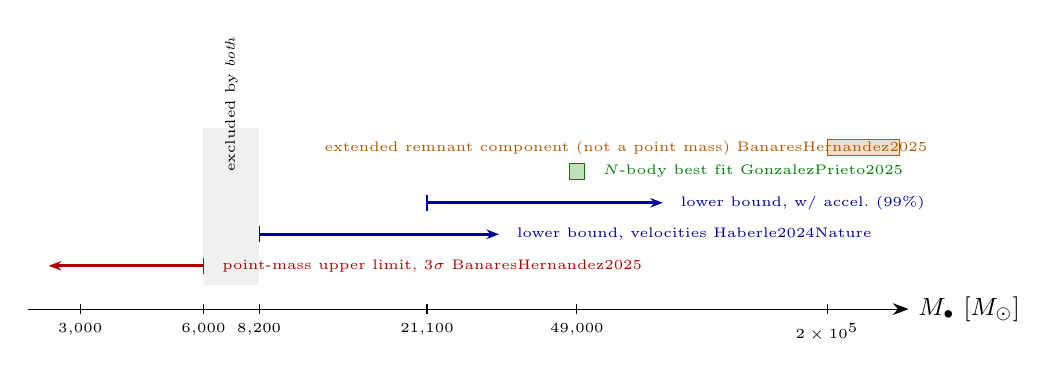
\begin{tikzpicture}[xscale=5.2]
% log10 mass axis from 3.4 to 5.4
\draw[-{Stealth[length=2mm]}] (3.35,0) -- (5.5,0) node[right, font=\small] {$M_{\bullet}$ [\msun]};
\foreach \x/\lab in {3.477/{$3{,}000$}, 3.778/{$6{,}000$}, 3.914/{$8{,}200$}, 4.324/{$21{,}100$}, 4.69/{$49{,}000$}, 5.301/{$2\times10^{5}$}}
  \draw (\x,0.06) -- (\x,-0.06) node[below, font=\tiny] {\lab};
% Banares upper limit: allowed below 6000
\draw[very thick, red!70!black, {Stealth[length=1.6mm]}-] (3.40,0.55) -- (3.778,0.55);
\draw[red!70!black] (3.778,0.45) -- (3.778,0.65);
\node[red!70!black, font=\tiny, anchor=west] at (3.80,0.55) {point-mass upper limit, $3\sigma$ \citep{BanaresHernandez2025}};
% Haberle velocities lower bound: allowed above 8200
\draw[very thick, blue!60!black, -{Stealth[length=1.6mm]}] (3.914,0.95) -- (4.50,0.95);
\draw[blue!60!black] (3.914,0.85) -- (3.914,1.05);
\node[blue!60!black, font=\tiny, anchor=west] at (4.52,0.95) {lower bound, velocities \citep{Haberle2024Nature}};
% Haberle accelerations lower bound
\draw[very thick, blue!60!black, -{Stealth[length=1.6mm]}] (4.324,1.35) -- (4.90,1.35);
\draw[blue!60!black] (4.324,1.25) -- (4.324,1.45);
\node[blue!60!black, font=\tiny, anchor=west] at (4.92,1.35) {lower bound, w/ accel.\ (99\%)};
% N-body band
\fill[green!50!black, opacity=0.25] (4.672,1.65) rectangle (4.708,1.85);
\draw[green!50!black] (4.672,1.65) rectangle (4.708,1.85);
\node[green!50!black, font=\tiny, anchor=west] at (4.73,1.75) {$N$-body best fit \citep{GonzalezPrieto2025}};
% Extended alternative band
\fill[orange!70!black, opacity=0.2] (5.301,1.95) rectangle (5.477,2.15);
\draw[orange!70!black] (5.301,1.95) rectangle (5.477,2.15);
\node[orange!70!black, font=\tiny, anchor=west] at (4.05,2.05) {extended remnant component (not a point mass) \citep{BanaresHernandez2025}};
% Conflict region shading
\fill[black, opacity=0.06] (3.778,0.3) rectangle (3.914,2.3);
\node[font=\tiny, rotate=90] at (3.846,2.6) {excluded by \emph{both}};
\end{tikzpicture}
\caption{The central-mass constraint landscape (logarithmic mass axis). The pulsar-timing point-mass upper limit and the fast-star kinematic lower bounds leave no allowed point mass: at least one constraint must yield. The exclusions are not symmetric: the timing limit applies to a \emph{point mass}, while the fast-star bounds apply to \emph{any} bound central mass interior to the fast-star orbits, so an extended remnant component evades the former but not the latter. The campaign is structured to determine which constraint yields, on a known schedule, using instruments that share no dominant systematics.}
\label{fig:massconstraints}
\end{figure}

\subsection{Three hypotheses, fixed in advance}
\label{sec:hypotheses}

Following Paper A we carry three competing hypotheses through every program:

\begin{description}
\item[$H_0$ (gas-starved IMBH or near-IMBH).] A genuine central point mass in the $\sim 10^{4}\,\msun$ range exists and is silent for the ordinary reason: a relaxed, gas-poor, 12-Gyr-old cluster supplies essentially nothing to accrete. Recent survival analyses find that IMBHs formed early in dense clusters are plausibly retained to the present day in \ocen-like hosts, supporting the prior on this branch \citep{Martinez2026}. Default and most parsimonious if the kinematic bounds hold.
\item[$H_1$ (extended remnant component).] No IMBH; the central mass is a spatially extended cluster of stellar remnants \citep{BanaresHernandez2025,BreenHeggie2013,Zocchi2019}. Default and most parsimonious if the timing bound holds.
\item[$H_2$ (anomalous/managed system).] A central IMBH whose observational properties are shaped by technology, per Paper A. Carries a low prior; becomes interesting only through conjunctions that $H_0$ and $H_1$ jointly fail to explain (e.g.\ near-extremal spin on a gas-starved hole; repeated coincident multi-messenger bursts; statistically anomalous depletion of the loosely bound core population).
\end{description}

The campaign's purpose is to measure the system well enough that $H_0$ and $H_1$ are decided on their merits, with $H_2$'s distinctive residues either appearing in the data or being retired by them, rather than to hunt for $H_2$. These labels map one-to-one onto the hypothesis set of the companion adjudication framework \citep[hereafter Paper E]{Swanson2026Engineered}: $H_0$ corresponds to Paper E's $H_q$ (quiescent astrophysical IMBH), $H_1$ to $H_{\rm sub}$ (sub-IMBH remnant alternative), and $H_2$ to $H_{\rm eng}$ (engineered system).

% =====================================================================
\section{Program 1: JWST infrared accretion and waste-heat limits}
\label{sec:jwst}

\paragraph{Bottom line.} Deep two-epoch JWST imaging of the core is the decisive observable: an accretion-like point source, or a mid-infrared excess over the stellar-population SED carrying the warm/cool swarm colour discriminant. The current best limits are archival: radiative output $\lesssim 10^{-9}$ of Eddington, radio accretion $\lesssim 4\times10^{-3}$ of the Bondi rate, and X-ray $L_{X} \lesssim 1.6\times10^{30}$~erg\,s$^{-1}$. The target sensitivity is $\sim$5--10~nJy ($3\sigma$) at F444W, a bolometric limit of order $10^{30}$~erg\,s$^{-1}$, and a tightened ceiling of $P_{\mathrm{comp}} \lesssim 10^{3}$--$10^{4}\,L_\odot$ on managed throughput. The result feeds the deepest multi-band quiescence statement available before LISA, and any excess or variability enters the coordination protocol of Section~\ref{sec:coordination}.

\subsection{Science case}

For any central mass $M_{\bullet}$, the Eddington luminosity is $L_{\rm Edd} \simeq 1.26\times10^{31}\,(M_{\bullet}/\msun)$~W: $1.0\times10^{35}$~W at $8{,}200\,\msun$, $2.5\times10^{35}$~W at $2\times10^{4}\,\msun$, $6.2\times10^{35}$~W at $4.9\times10^{4}\,\msun$. The existing non-detections already establish extreme quiescence: the radio limit bounds accretion at $\lesssim 4\times10^{-3}$ of the Bondi rate \citep{Mahida2026}, the archival Chandra limit bounds the X-ray output at $L_X \lesssim 1.6\times10^{30}$~erg\,s$^{-1}$ \citep{Haggard2013}, and the JWST photometry bounds the radiative output at $\lesssim 10^{-9}$ of Eddington \citep{Chen2025JWST}, among the most extreme quiescence levels measured for any black hole. The published JWST analysis, however, is an archival by-product rather than an optimized deep program, and the gain a purpose-designed campaign buys depends on which quantity is being compared. In flux the deep program improves on Chen et al.'s own archival depths by 22$\times$ at F770W and 39$\times$ at F1000W before crowding, and by 7.4$\times$ and 13$\times$ after the adopted penalty. In Eddington ratio the gain is far larger, from the $\lesssim 10^{-9}$ the archival photometry supports to $4\times10^{-14}$--$4\times10^{-13}$ at $2\times10^{4}\,\msun$, a factor $2.5\times10^{3}$ to $2.5\times10^{4}$, because the bolometric conversion is not the same at the two depths. The two figures are quoted separately here, since ``an order of magnitude'' matches neither. The archival $\lesssim 10^{-9}$ anchor is itself a bolometric reading of \citet{Chen2025JWST}: their F444W depth converts to $\sim$$4\times10^{-12}$ of Eddington monochromatically, and the looser published figure carries their SED assumption rather than ours. The deep program adds the two dimensions the archival data lack: variability (accretion at these rates is expected to flicker; a managed or artificial suppression of accretion, the $H_2$ residue, is not) and waste heat (a mid-infrared excess over the stellar population model is the classic Dyson-type technosignature; \citealt{Dyson1960,Wright2014,Hsiao2021}, and at \ocen{} the relevant solid angle is a few arcseconds, not a galaxy).

\subsection{Current and scheduled JWST programs}
\label{sec:jwstexisting}

Two approved JWST programs already execute pieces of this campaign, and the deliverables below are stated as increments over them. GO 5137 (PI Seth), ``Weighing the Intermediate Mass Black Hole in Omega Centauri,'' obtains a deep NIRSpec IFU mosaic of the central field: line-of-sight (LOS) velocities for $\sim$70 stars in the innermost region, including all four fast movers inside $1''$, together with the deepest search to date for accretion-emission signatures at the candidate position \citep{JWSTGO5137}. GO 8322 extends the astrometric time base with dedicated JWST monitoring of the fast stars \citep{JWSTGO8322}. That changes three things for Program 1: (i) the accretion-emission search is no longer virgin territory --- the deep-imaging deliverable is the order-of-magnitude \emph{photometric} depth gain, the second epoch for variability, and the 10--25.5~$\mu$m waste-heat axis (the long-wavelength limit of MIRI imaging), none of which the IFU program provides; (ii) the contingent spectroscopic environment test (below) becomes an extension of GO 5137's footprint rather than a first observation; and (iii) the LOS velocities feed directly into the astrometric program, where they convert two-dimensional proper motions into three-dimensional velocity vectors and open a radial-velocity acceleration channel (Section~\ref{sec:honest}).

\subsection{Implementation}

\textbf{Deep imaging (new observations).} NIRCam F200W/F356W/F444W at 20~ks per filter plus MIRI F770W/F1000W at 15~ks per filter, in two epochs separated by $\sim$6 months: $\sim$65~h total. In the crowded core the limits are confusion- rather than photon-limited. The NIRCam figures are ETC-class point-source depths scaled to the requested 20~ks exposure and degraded by an assumed $\sim$2.9$\times$ crowding penalty, reaching $\sim$5--10~nJy ($3\sigma$) across F200W/F356W/F444W; the empirical-PSF-subtraction gain, anchored to the oMEGACat astrometric catalogue \citep{Haberle2024oMEGACatII,Nitschai2023}, is named as an assumption to be verified by scene simulation, not a measured recovery. Chen et al.'s own archival NIRCam photometry of this field reaches 660~nJy--1.6~$\mu$Jy at their 515~s exposure \citep{Chen2025JWST}, which implies a crowding penalty of $\sim$29--70$\times$ without PSF subtraction and puts the adopted $\sim$2.9$\times$ assumption in view as an assumption rather than a demonstrated anchor. At MIRI the ETC-class point-source depths at 15~ks are $\approx$70~nJy ($3\sigma$) at F770W and $\approx$170~nJy at F1000W before crowding, degrading to $\approx$200 and $\approx$500~nJy respectively after the crowding penalty discussed next. At the \ocen\ core stellar density ($\rho_{0} \simeq 3\times10^{3}$\,\msun\,pc$^{-3}$; $\sim$$10^{7}$ stars in the field) the NIRCam F444W pixel scale ($0.063^{\prime\prime}$) resolves of order fifty stars per resolution element in the inner arcsecond, and the 90\,per\,cent injection depth is a property of the local surface density and the PSF-fitting algorithm rather than the instrument. Table~\ref{tab:jwst-perfilter} breaks the scalar $\sim$3 crowding factor into per-filter completeness versus photon limits, using the same Chen et al.\ 90\,per\,cent completeness curves that set the Paper~F infrared leg (their Table~1, scaled by exposure time; Paper~F Appendix~\ref{app:conventions} and \texttt{miri\_sensitivity.json}, ETC\,6.0). For each filter the ETC photon-limited 3$\sigma$ depth at the requested exposure and the 90\% injection-recovery depth are compared; the adopted depth is the shallower. At the requested 20\,ks (NIRCam) and 15\,ks (MIRI) the completeness depth is shallower in every filter, so the program is crowding-limited and its exposure is sized to that wall (Table~\ref{tab:jwst-perfilter}). Doubling the integration improves the photon limit by $1/\sqrt2$ but moves the adopted limit by ${<}0.1$\,dex, while halving it would make sensitivity bind. This pre-empts the TAC question of why 15\,ks rather than 8\,ks at MIRI: at 8\,ks the photon and completeness depths are comparable, and at 15\,ks the photon depth sits a factor $\sim$1.5 below the completeness wall, so the time request buys the wall rather than empty depth. The MIRI figures carry the larger systematic: RGB-tip giants are mJy-level sources at 10\,$\mu$m whose extended PSF halos overlap in the core, in-flight long-wave throughput degradation must still be budgeted, and the quoted depths assume the NIRCam-calibrated $\sim$3$\times$ penalty transfers to the mid-IR PSF---assumptions a full scene simulation must verify before the time request is finalized.

\begin{table}[htbp]
\centering
\small
\caption{Per-filter depth at the requested exposure: photon limit versus 90\% completeness (Chen et al.\ 2025, as used in Paper~F) and which binds. MIRI ETC from \texttt{miri\_sensitivity.json} (ETC~6.0, 10\,ksec scaled as $t^{-1/2}$; rescaled 61\,nJy at F770W and 115\,nJy at F1000W 3$\sigma$, printed as $\approx$70 and $\approx$170\,nJy before crowding); NIRCam ETC/completeness from the oMEGACat F444W injection that recovers 90\% at the quoted depth, scaled by exposure and pixel scale with F356W interpolated. Adopted is the shallower; all five filters are crowding-limited at the requested depth, so exposure is sized to the completeness wall.}
\label{tab:jwst-perfilter}
\begin{tabular}{lccrrcl}
\toprule
Filter & $\lambda_{\rm piv}$ ($\mu$m) & Exp.\ (ks) & ETC photon $3\sigma$ (nJy) & 90\% completeness (nJy) & Binds & Adopted $3\sigma$ (nJy) \\
\midrule
F200W  & 2.00 & 20 & 4 & 12 & crowding & 12 \\
F356W  & 3.56 & 20 & 3 & 9 & crowding & 9 \\
F444W  & 4.44 & 20 & 3 & 8 & crowding & 10\textsuperscript{a} \\
F770W  & 7.70 & 15 & 61 (70\textsuperscript{b}) & 184 (200\textsuperscript{b}) & crowding & 200 \\
F1000W & 10.0 & 15 & 115 (170\textsuperscript{b}) & 345 (500\textsuperscript{b}) & crowding & 500 \\
\bottomrule
\multicolumn{7}{l}{\footnotesize \textsuperscript{a} Printed as $\sim$5--10\,nJy (3$\sigma$) across F200W/F356W/F444W, anchored to the injection; adopted 10\,nJy is the} \\
\multicolumn{7}{l}{\footnotesize \phantom{\textsuperscript{a}} shallower end, consistent with $3\times$ penalty. \textsuperscript{b} Parentheses are the values quoted in} \\
\multicolumn{7}{l}{\footnotesize \phantom{\textsuperscript{a}} the pre-table sentence; they exceed the rescaled figures by 14\% at F770W and 48\% at} \\
\multicolumn{7}{l}{\footnotesize \phantom{\textsuperscript{a}} F1000W, which is a conservative round-up rather than a rounding. The adopted column takes} \\
\multicolumn{7}{l}{\footnotesize \phantom{\textsuperscript{a}} the shallower quoted value in each case; first numbers are the rescaled ETC/completeness} \\
\multicolumn{7}{l}{\footnotesize \phantom{\textsuperscript{a}} from \texttt{fC\_calc7\_miri.json}.} \\
\end{tabular}
\end{table} At 5.49~kpc, 10~nJy at F444W corresponds to a monochromatic $\nu L_{\nu} \approx 2.5\times10^{28}$~erg\,s$^{-1}$; for plausible quiescent-accretion SEDs the bolometric limit is of order $10^{29}$--$10^{30}$~erg\,s$^{-1}$, i.e.\ Eddington ratios of $4\times10^{-14}$--$4\times10^{-13}$ at $2\times10^{4}\,\msun$, probing a regime in which even Sgr~A* would be conspicuous \citep{EHT2022SgrAI}.

\textbf{Two-epoch variability.} Differential photometry between epochs is robust to the static crowding systematics that dominate the absolute limits, and the trigger is a significance on the epoch difference rather than an amplitude alone. Two epochs at per-epoch $1\sigma$ noise $\sigma_{1}$ give a difference noise $\sqrt{2}\,\sigma_{1}$, so an amplitude $f$ on a source of flux $F$ is detected at $fF/(\sqrt{2}\sigma_{1})$. At the adopted NIRCam depth ($10$~nJy at $3\sigma$, so $\sigma_{1} = 3.3$~nJy and $\sqrt{2}\sigma_{1} = 4.7$~nJy) a $3\sigma$ difference at 20 per cent amplitude needs $F > 71$~nJy, and $47$~nJy at 30 per cent; at the post-crowding F1000W depth ($500$~nJy at $3\sigma$) the corresponding floors are $3.5\,\mu$Jy and $2.4\,\mu$Jy. Draft v2.6's ``$\geq$20--30 per cent for any source above $\sim$30~nJy at NIRCam (above $\sim$0.5~$\mu$Jy at F1000W)'' is withdrawn: those fluxes give $1.3\sigma$ and $0.42\sigma$ at 20 per cent amplitude, so they would promote noise. The pre-registered trigger is a $5\sigma$ difference, which at 20 per cent amplitude requires $F > 118$~nJy at NIRCam and $F > 5.9\,\mu$Jy at F1000W, and the floors degrade further by the per-filter crowding penalty of Table~\ref{tab:jwst-perfilter}, which the F1000W figure already carries and the NIRCam figure does not. Any source clearing that threshold flags an accretion candidate and triggers the coordination protocol of Section~\ref{sec:coordination}. Two-epoch photometry should not be mistaken for a test of Paper E's regulation statistic $R$, the variability \emph{deficit} in the MAD flux-eruption band ($10^{-3}$--$10^{-1}$~Hz for a $2\times10^{4}\,\msun$ hole; cycle times of 10--100~s), which requires fast-cadence monitoring. At the fiducial mass that is an X-ray measurement, not a radio one: a compact self-absorbed synchrotron source low-pass filters the eruption band at the source, and interstellar scintillation adds variability uncorrelated with accretion on top, so the radio band carries no discriminating power for $R$; the channel activates at $L_X \gtrsim 10^{34}$--$10^{35}$~erg\,s$^{-1}$, i.e.\ in flare or TDE states \citep{Swanson2026Engineered}. Accordingly, if accretion is ever detected at that level in any band, a fast-cadence X-ray contingency activates (pointed timing plus the archival X-ray channel of Program 8), targeted at the eruption band, with Program-2 radio monitoring serving as context rather than as an $R$ measurement.

\textbf{Waste-heat analysis (archival + new).} The 10--25.5~$\mu$m field photometry is fitted against the synthetic stellar-population SED constructed from the oMEGACat spectroscopic catalogue \citep{Nitschai2023}. The primary waste-heat deliverable is a \emph{point-source} SED excess with a colour discriminant: the configurations surviving Paper E's feasibility analysis are cool swarms at $10^{2}$--$10^{3}$~AU, which subtend $0.018''$--$0.18''$ at 5.49~kpc and are unresolved inside the F1000W PSF core ($0.33''$), so morphology carries no information inside that envelope and the discriminant is spectral: a 50--300~K near-blackbody with no silicate features, against the AGB dust shells that dominate the false-positive population \citep{Swanson2026Engineered}. Paper E's swarm SED forward model (Appendix~C as of v2.1, ``Priors, likelihoods, and computation''; retrace by content, not appendix letter, if Paper E's appendix order changes again), a two-temperature swarm SED integrated against the nine MIRI imaging filters, supplies this discriminant quantitatively: any point-source excess is tested against the predicted warm/cool flux ratio across F560W--F2550W rather than a single-band flux, which any AGB dust shell of comparable brightness will not reproduce over the same filter set. We retain the extended statistic (a spatially coherent excess in the central $0.1$~pc, i.e.\ $3.8''$, exceeding $3\sigma$ over the population model) but relabel it: it is a hypothesis-agnostic anomaly channel, no longer the test of the surviving waste-heat configurations. The deliverable is quantitative through Paper E's waste-heat floor, $L_{\rm waste} \geq 10^{-4}\,P_{\rm comp}$: the current JWST-derived limit converts to a ceiling on sustained computational power of $P_{\rm comp} \lesssim 10^{3}$--$10^{4}\,L_\odot$, and the ceiling tightens linearly with mid-infrared depth \citep{Swanson2026Engineered}. One temperature qualifier bounds every MIRI-derived ceiling: a 50~K swarm peaks near 60~$\mu$m and is essentially invisible at $\leq 25.5~\mu$m, so the ceiling applies to the warm ($\gtrsim 150$~K) end of the configuration space only, and the cold end is unconstrained by any instrument in this campaign. The same fit yields conventional science: the most precise mid-IR census of the post-main-sequence population in any globular cluster.

\textbf{Spectroscopic environment test (Cycle 6+, contingent).} The approved GO 5137 IFU observations (Section~\ref{sec:jwstexisting}) already cover the innermost arcseconds; the contingent extension proposed here is a wider NIRSpec IFU mosaic of the inner $0.5$~pc ($\sim$125~h), activated only if astrometry or timing strengthens the IMBH case, mapping abundance anomalies (Li enhancement, refractory depletion) that would discriminate between ordinary tidal-disruption debris chemistry \citep{Hills1988,Gezari2021} and the engineered-feeding residue of $H_2$. We do not request this time until the trigger condition is met.

\subsection{Decision criteria}

Null result (expected under $H_0$, $H_1$, and mature-$H_2$ alike): bolometric limit $\lesssim 10^{30}$~erg\,s$^{-1}$ recorded (radiative output $\lesssim 10^{-12}$ of Eddington across the contested mass range), complementing the radio Bondi-efficiency bound and jointly constraining any radiatively inefficient flow via the fundamental plane \citep{Merloni2003,Mahida2026}. A static detection consistent with a quiescent accretion SED supports $H_0$ and immediately sharpens every dynamical program (the source position becomes the kinematic centre). A variable detection triggers multi-messenger follow-up. A $>3\sigma$ mid-IR excess (point-source with the swarm colour discriminant, or extended with no stellar counterpart) is the single strongest electromagnetic anomaly the campaign can produce and would be adjudicated under Section~\ref{sec:coordination} rules.

% =====================================================================
\section{Program 2: radio deep imaging, narrowband SETI, and pulsar timing}
\label{sec:radio}

\paragraph{Bottom line.} The decisive observable is the radial profile of millisecond-pulsar accelerations across the cluster, which distinguishes a central point mass from an extended remnant component; the narrowband SETI limit and the deeper continuum image ride on the same sessions. The current best limits are the $3\sigma$ point-mass cap of $\sim6\times10^{3}\,\msun$ from the joint kinematic-timing analysis and the latest joint MeerKAT--Parkes insensitivity at $10^{3}$--$10^{4}\,\msun$ with a $90$-per-cent ceiling of $10^{5}\,\msun$. The target is ten well-timed pulsars on ten-year baselines, pushing the bound to the $3{,}000$--$4{,}000\,\msun$ level or finding the profile, plus a first \ocen{} technosignature limit near $4\times10^{15}$~W EIRP over the full cluster. This program feeds decision point D2 directly.

\subsection{Science case}

The radio program carries three loads at once. (i) \emph{Continuum}: a deeper interferometric limit (or first detection) on the central compact source, extending \citet{Mahida2026} and the globular-cluster IMBH radio campaigns \citep{Strader2012,Tremou2018}. (ii) \emph{Narrowband SETI}: to our knowledge the first dedicated technosignature search of any kind at \ocen{}, closing the gap left by the FAST pilot survey's latitude limit \citep{Huang2026}. (iii) \emph{Pulsar timing}: the binding constraint on the central mass comes from the cluster's MSP population (five discovered with Parkes, \citealt{Dai2020}, timed to $\dot\nu$ within 3.5~yr, \citealt{Dai2023}; then thirteen more with MeerKAT/TRAPUM, \citealt{Chen2023,StappersKramer2016}). The joint MeerKAT--Parkes timing analysis now extends both the census and the constraints: it reports a nineteenth discovery, PSR J1326$-$4728S, bringing the known population to nineteen, and its measurements are insensitive to an IMBH of $10^{3}$--$10^{4}\,\msun$ while placing a 90 per cent upper limit of $<10^{5}\,\msun$ on the central mass \citep{ColomiBernadich2026}. The same analysis finds an anomalously high fraction of isolated and black-widow systems among the cluster's MSPs, which bears directly on the MSP radial-distribution priors on which the \citet{BanaresHernandez2025} timing bound leans, since the spatial distribution of a dynamically processed population need not follow the assumed profile. The path to resolving the mass tension runs directly through more pulsars and longer baselines \citep{BanaresHernandez2025,Chen2025MiniPTA}.

\subsection{Implementation: MeerKAT era (2026--2030)}

\textbf{Timing.} Bi-weekly L-band sessions ($\sim$26 per year, $\sim$3--5~h each) on all nineteen MSPs with MeerKAT \citep{Jonas2016}, producing times of arrival at several-$\mu$s precision for the brightest objects (the cluster's MSPs are 10--30~$\mu$Jy sources; sub-$\mu$s timing is not on offer). Line-of-sight acceleration precision from timing scales steeply with baseline ($\sigma_{a}\propto T^{-5/2}$ for white noise); by analogy with the mature 47~Tuc and Terzan~5 programs \citep{Freire2017,Prager2017}, five years of MeerKAT data yield per-pulsar acceleration uncertainties of order $10^{-10}$~m\,s$^{-2}$ for the best-timed objects. We do not extrapolate to the $10^{-11}$ decade: the 47~Tuc and Terzan~5 precedents rest on 20--25-yr baselines, and DM variation and red timing noise break the white-noise $T^{-5/2}$ scaling before that precision is reached \citep{VanHaasteren2013}. For scale, a $4\times10^{4}\,\msun$ point mass imposes $a \approx 6\times10^{-8}$~m\,s$^{-2}$ at $r=0.3$~pc: the discriminating signal is not the detection of acceleration (already achieved; \citealt{Dai2023,BanaresHernandez2025}) but the radial profile of accelerations and jerks across the MSP population, which distinguishes a point mass ($a \propto r^{-2}$) from an extended remnant component. Commensal search observations are expected to add 5--10 MSPs (the luminosity function is far from exhausted; \citealt{Chen2023}), and the population-level point-mass upper bound tightens approximately as $1/\sqrt{N_{\mathrm{eff}}}\,(T_0/T)^{\,\geq 1}$; this is an ensemble, bound-level scaling, distinct from the per-pulsar white-noise acceleration scaling $\sigma_{a}\propto T^{-5/2}$ quoted above, because the ensemble constraint is limited by the pulsars' unknown line-of-sight positions and intrinsic spin-down as well as by timing noise. The effective sample size is not 19. The released timing record (\texttt{paper/h/data/pulsars.json}) carries published timing solutions for twelve of the nineteen pulsars: seven (A, B, C, D, E, H, K) on the full Murriyang UWL campaign, 2020 April 1 to 2025 May 20, a 5.13-yr baseline, and five (G, I, L, N, Q) on MeerKAT-only solutions spanning 2021--2025, taken as 4.0~yr. Six others (F, J, M, O, P, R) have no timing solution in the record and one more (S) is a single-epoch discovery. The per-pulsar acceleration sensitivities, $\sigma_{a,i} \propto P_{i}\,\sigma_{t,i}/T_{i}^{2}$, differ through the spin periods (2.5--19~ms), so the inverse-quadrature sum with weights $w_{i} = 1/\sigma_{a,i}$ gives $N_{\mathrm{eff}} = (\sum_{i} w_{i})^{2}/\sum_{i} w_{i}^{2} = 10.0$ on that baseline assignment, replacing the $9.8$ carried through Draft v2.6, which stated no baselines and was therefore not reproducible. Two other readings of the same twelve bracket it: weighting by baseline alone gives $11.4$, and equal weights give $12$. The timing residual enters $\sigma_{a,i}$ as a common factor (several-$\mu$s ToA precision, not sub-$\mu$s) and cancels in $N_{\mathrm{eff}}$, which is a ratio of weight moments; rescaling every $\sigma_{t,i}$ by a common constant leaves $N_{\mathrm{eff}}$ unchanged to machine precision, as \texttt{paper/figs/fC\_r9\_checks.py} verifies. The spin period does not cancel and is not claimed to. The ensemble sensitivity is dominated by the seven pulsars on the longer baseline, the shortest-period of which (H, 2.52~ms) alone carries 17 per cent of the total weight. Ten well-timed pulsars with ten-year baselines push a $6{,}000\,\msun$ bound to the $3{,}000$--$4{,}000\,\msun$ level if no point-mass signal emerges, or find one. That forecast and \citet{ColomiBernadich2026}'s statement that the present measurements are insensitive to $10^{3}$--$10^{4}\,\msun$ are consistent rather than contradictory: the insensitivity is a statement about the current 4--5-yr baselines, and the projection buys its factor from doubling the baseline against the $T^{-5/2}$ per-pulsar scaling and from the ensemble term, with the reservations on red noise and DM variation above. The projection is a forecast on this paper's own account and is not attributed to that analysis.

\textbf{Forecast requirement (pre-registered).} The profile discriminator just described is the campaign's primary near-term test, and it is at present asserted rather than demonstrated: most of the MSPs sit well outside the central 0.1~pc, and their unknown line-of-sight positions degrade the radial information the test needs. Before the D2 data lock (decision point D2 of the D1--D4 sequence defined in Section~\ref{sec:decision}) we will therefore complete and publish a mock-population forecast: point-mass and extended-component potentials injected at the real MSP sky positions, line-of-sight positions marginalized over the cluster density profile, and realistic timing noise applied, reporting the recoverable Bayes factor (or $\Delta\chi^{2}$) as a function of baseline and census size. An order-of-magnitude expectation frames the exercise: with 19--25 MSPs, 5--10-yr baselines, and per-pulsar acceleration uncertainties of order $10^{-10}$~m\,s$^{-2}$, the profile difference between a $2\times10^{4}\,\msun$ point mass and a $2$--$3\times10^{5}\,\msun$ extended component is of order $10^{-9}$--$10^{-8}$~m\,s$^{-2}$ for the innermost pulsars at their favourable, near-plane-of-sky assumed 3D positions. The pre-registered success criterion is a median discrimination of $\Delta\chi^{2}\geq 9$ between the two named potentials at the D2 epoch; if the forecast falls short, the D2 decision weight shifts to the astrometric channels of Section~\ref{sec:astrometry}.

\textbf{Forecast as executed.} The forecast has been run (\texttt{paper/figs/fC\_calc7b\_d2forecast\_v2.py}; 200 realizations per cell, three injected truths $\times$ five noise floors $\times$ four census sizes). The forecast returns two statistics, and they behave differently enough that quoting one without the other misrepresents the test. Both are signed positive toward the extended potential throughout. The \emph{fixed-parameter} statistic compares the two named potentials with no free parameters, and it is the one D2 routes on: under the injected $2\times10^{4}\,\msun$ point mass its median is $-93$ to $-419$ across the noise ladder at the current census of nineteen, and it routes to the point-mass branch in every realization of every cell; under the injected $2.5\times10^{5}\,\msun$ extended component the medians run $+1.1\times10^{4}$ to $+4.7\times10^{7}$ and it routes to the extended branch equally reliably. The \emph{free-parameter} statistic, which maximises each family over its own mass (and, for the extended family, scale) grid, cannot be used for routing at all: under the point-mass truth its median is $+79$ at the timing-limited floor and stays positive down to $+1.3$ at three times Paper H's budget, favouring the extended family whichever family is true, and it recovers the correct sign in only 11--18 per cent of realizations. The reason is structural rather than a defect of implementation. The extended family reduces to the compact one as its scale radius goes to zero, so maximising over the larger family can only improve the fit; the statistic measures fit improvement and carries no information about which model generated the data. The order-of-magnitude ``$\Delta\chi^{2}$ of order tens ($\ln K \sim 5$--$15$)'' expectation carried through Draft v2.6 corresponds to nothing the forecast returns for either statistic, and is withdrawn in favour of the numbers above.

The equivalence $\Delta\chi^{2} = 2\ln K$ holds only when the two models being compared have the same dimension, and it is retracted here for the free-parameter case: the extended family carries one extra parameter, and at the current census the free-parameter $\Delta\chi^{2}$ and $2\ln K$ differ by 5 per cent at the timing-limited floor ($+79.2$ against $+75.1$) and disagree in sign at the noisiest ($+1.25$ against $-1.32$). It remains exact for the fixed-parameter statistic, which is why the routing thresholds are stated on that one.

\textbf{Where the test has no authority.} Both named potentials differ in enclosed mass within the pulsar region by a factor of 12.5, so a statistic distinguishing them is partly reading mass rather than profile shape. A third truth isolates this: a Plummer component of $3.3\times10^{4}\,\msun$ at $a = 2$~pc, chosen to enclose the same mass as the $2\times10^{4}\,\msun$ point mass at the median projected pulsar radius (3.13~pc). The routing statistic recovers it at the two deepest noise floors (routes correctly in 100 and 99 per cent of realizations at $3.09$ and $10$ (km\,s$^{-1}$)$^{2}$\,pc$^{-1}$), and then fails: at $31.6$ and above the median turns negative and it routes a genuinely extended component to the point-mass branch in 91 per cent of realizations, rising to 100 per cent at the two highest floors. D2's authority is therefore limited to discriminating the two potentials it names. An extended component whose enclosed mass resembles the point mass is misrouted at the realistic noise floors, and that limitation is carried into the routing rule of Amendment~C-A1 rather than left implicit. A complementary dynamical diagnostic is available from the same data: an IMBH measurably alters the degree of energy equipartition of the host cluster \citep{ArosVesperini2023}, so the equipartition profile inferred from the kinematic catalogues provides an independent axis along which the point-mass and extended hypotheses separate.

\textbf{Narrowband SETI.} Commensally with every timing session, a 1-Hz-resolution spectrometer backend records the full primary beam (FWHM $\sim 1^{\circ}$ across most of L band, containing the whole cluster). Processing follows standard drift-search practice \citep{Enriquez2017}: Doppler drifts of $\pm 4$~Hz\,s$^{-1}$ at L band (a fractional convention, $\dot\nu/\nu \approx 3\times10^{-9}$~s$^{-1}$; the absolute window scales with observing frequency for any S-band search), on--off cadence against reference pointings, and a candidate-advance threshold of SNR~$>15$. The sensitivity limits below are quoted at the conventional $\mathrm{SNR}=10$ of Eq.~(\ref{eq:eirp}); the two numbers serve different roles (limit-setting versus pipeline promotion) and are stated separately to keep them from being conflated. Seventy hours over two years reach a minimum detectable EIRP of $\sim 4\times10^{15}$~W at 5.49~kpc. Deeper is available on the same commensal data at no extra facility cost, since the limit improves as $t^{-1/2}$: the full five-year timing allocation accumulates 156--260~h and lowers the threshold by a factor 1.5--1.9 (to $\sim 2$--$3\times10^{15}$~W). The 70-h figure is the two-year milestone quoted for the first publication, and the five-year figure is the programme's end state. That threshold follows from the standard narrowband relation
\begin{equation}
\mathrm{EIRP}_{\min} \;=\; 4\pi d^{2}\,\mathrm{SNR}\;\mathrm{SEFD}\,\sqrt{\delta\nu/t},
\label{eq:eirp}
\end{equation}
with $d = 5.49$~kpc, $\mathrm{SNR} = 10$, $\delta\nu = 1$~Hz, and $t = 70$~h. The SEFD entering Eq.~(\ref{eq:eirp}) is an array figure, not an antenna figure: the $\approx 430$~Jy value is the per-antenna SEFD of a single 13.5-m MeerKAT dish \citep{Jonas2016}, and an $N \approx 60$-antenna sum improves on it by $\sqrt{N}$ to $\approx 55$~Jy incoherently, or by $N$ to $\approx 7$~Jy in a coherent tied-array beam. The quoted $4\times10^{15}$~W is the incoherent, full-cluster figure; a coherent tied-array pointing reaches $\approx 5\times10^{14}$~W but covers only an arcseconds-scale beam. These limits are quoted within the half-light radius: the EIRP limit degrades by $2\times$ at the half-power radius of the primary beam, a transmitter at the $\sim$0.8--1$^{\circ}$ tidal radius (Harris catalogue 1.06$^{\circ}$, \citealt{Harris1996}; a Nature-paper King-profile fit gives 0.81$^{\circ}$, \citealt{Haberle2024Nature}) sits at or beyond the half-power point at the top of L band, and the S-band primary beam ($\sim 40'$) does not contain the cluster at all. The incoherent full-cluster limit is below the FAST pilot's $\sim 10^{16}$~W thresholds at its closer, northern targets \citep{Huang2026}; it is the first limit of any kind for this cluster, and it is sufficient to detect any transmitter exceeding $\sim 2\times10^{2}$ times the EIRP of the Arecibo planetary radar ($\sim 2\times10^{13}$~W; \citealt{Enriquez2017}, a modest output for an energy-rich civilization) from any of $\sim 10^{7}$ stars in the beam simultaneously. For comparison with FAST's per-target accounting, a single $5''$ coherent follow-up beam at the core contains $\sim 10^{3}$ stars, so even the deep coherent limit is a per-thousand-star figure rather than a per-star one.

\textbf{Backend requirement: spatial RFI discrimination.} An incoherent full-primary-beam sum has no spatial discrimination: every signal within $\sim1^{\circ}$ enters the data product, and there is no on/off inside a single pointing. The dominant contaminant for a 2026+ campaign is not fixed-frequency terrestrial RFI but LEO mega-constellation downlinks sweeping through L band with Doppler drifts inside the searched $\pm 4$~Hz\,s$^{-1}$ window; candidate rates of $10^{4}$--$10^{5}$~hr$^{-1}$ are routine in current data. The mitigation is architectural rather than procedural: simultaneous coherent beams with candidate cross-rejection, the BLUSE architecture of \citet{Czech2021}, in which a candidate appearing in widely separated beams is rejected as local. Tiling the half-light region with $5''$ coherent beams would require thousands of beams; the realistic design forms a modest set of anti-coincidence beams plus a reduced-baseline subarray whose wider coherent beams cover the core at intermediate SEFD. We state this as a hard backend requirement, because without it the false-candidate budget, not the radiometer equation, sets the program's labour cost.

\textbf{Scintillation-aware confirmation.} The 5.49-kpc, DM~$\approx 100$~pc\,cm$^{-3}$ sightline scintillates strongly at L band: diffractive scintillation modulates a narrowband signal by factors of several on minutes-to-hours timescales, the case treated for SETI by \citet{CordesLazioSagan1997}. A criterion requiring re-detection in a single independent session would therefore reject a genuine steady transmitter with order-unity probability whenever the confirming epoch lands in a scintillation null. The pre-registered confirmation policy is scintillation-aware: a candidate surviving the cross-rejection screen is scheduled for multiple re-observation epochs spaced by at least the refractive timescale, and confirmation significance is computed under exponential-intensity statistics rather than a constant-flux assumption, so that a non-detection in any single epoch demotes rather than kills the candidate.

\textbf{Continuum.} The summed continuum visibilities from the timing campaign provide a $\sim$100+~h synthesis dataset at L/S band, and the depth budget is set by confusion, not thermal noise: at the $\sim6''$ resolution of a naturally weighted L-band image the
confusion limit is formalism-dependent: the classical one-source-per-beam
criterion gives $\approx0.35$~$\mu$Jy, while the Condon (1974)
self-consistent criterion (cutoff at five times the rms confusion;
\citealt{Condon2007}) gives $\approx3.5$~$\mu$Jy, against a thermal
noise of 0.41~$\mu$Jy in 100\,h (Table~\ref{tab:confusion}). The
confusion-versus-thermal ordering at $6''$ therefore depends on the
formalism, while at UHF confusion dominates in both; 19+ steep-spectrum MSPs
sit at the position of interest either way. The useful deliverables are therefore long-baseline, uniform-weighted imaging of the central arcminute (where the confusion limit is far deeper), UHF/S-band spectral decomposition separating the steep-spectrum pulsar population from any flat-spectrum accretion candidate, and in-beam variability of compact sources; combined with the ATCA 7.25-GHz limit \citep{Mahida2026} these constrain both the flat-spectrum (jet) and steep-spectrum (pulsar) interpretations of any future central source candidate.

\subsection{Implementation: SKA era (2029--)}

SKA-Mid science verification is expected from 2027, shared-risk operations from 2029, and early full operational cycles in the early 2030s \citep{Braun2019SKA}. The \ocen{} program transfers wholesale: timing precision improves by the sensitivity ratio (factor $\sim$4--5 over MeerKAT for these declinations), the MSP census plausibly doubles, and the narrowband EIRP thresholds drop by the same factor, toward $\sim 10^{15}$~W incoherent and $\sim 10^{14}$~W coherent, on a southern target FAST cannot see. (The ngVLA, the other next-decade radio flagship, is not an option here: at $\delta = -47.5^{\circ}$ \ocen{} is inaccessible from its planned sites.) By LISA launch, the pulsar acceleration map will be the best non-GW constraint on the central potential in any globular cluster.

\subsection{Decision criteria}

The timing program is the campaign's primary near-term discriminator between $H_0$ and $H_1$: a smooth $r^{-2}$ acceleration profile centred on the kinematic centre to within $\max(1'', r_{\bullet}(M_{\bullet}))$, the wander-inflated tolerance of Section~\ref{sec:wander}, at $\geq 10^{4}\,\msun$ retires $H_1$; a persistently tightening upper bound below the kinematic lower bounds forces revision of the fast-star analysis (membership, foreground, or binarity systematics) and shifts the campaign's centre of gravity to $H_1$. For SETI: any re-detected narrowband candidate enters the two-messenger protocol; a null is published as the first \ocen{} technosignature limit. Paper A dependence (labelled): under $H_2$, P3 of that paper predicts no leakage radiation, so SETI nulls carry no evidential weight against $H_2$; they constrain only conventional beacon scenarios. Consistent with this, Paper E's Bayes-factor analysis finds that additional radio depth beyond current limits moves $\ln K$ only weakly for every hypothesis pairing \citep{Swanson2026Engineered}; the case for the deeper continuum limit therefore rests on the $H_0$/$H_1$ accretion physics, not on technosignature discrimination.

\subsubsection{Confusion per band}
\label{app:confusion}
Classical confusion estimates differ by about an order of magnitude at these
resolutions depending on formalism, so Table~\ref{tab:confusion} carries the
two defensible readings per band rather than one number: the
one-source-per-beam cutoff at half its flux, and the Condon self-consistent
criterion, whose cutoff sits at five times the rms confusion
\citep{Condon2007}; the framework is the flux-density error-distribution
formalism of \citet{Condon1974}. Both readings use the same deep 1.4-GHz
count law
($N(>S) \approx 220\,(S/\mathrm{mJy})^{-1}$\,deg$^{-2}$ across
10\,$\mu$Jy--1\,mJy, flattening toward the Euclidean slope above 1\,mJy),
whose normalization carries about a factor-of-two uncertainty; the band-to-band
ratios are more robust than the absolute scale. The independent cross-check
supports that factor and no better: \citet{Vernstrom2014} measure an rms
confusion of $\sim$1.2~$\mu$Jy\,beam$^{-1}$ at 3~GHz and $8''$, where the
count law and criterion adopted here give 2.8~$\mu$Jy\,beam$^{-1}$. The
spread is therefore a factor of ten within a band and a factor of sixty
across the table (0.15 to 9.1~$\mu$Jy\,beam$^{-1}$), and the absolute scale
is not settled by anything in this paper. Which column binds depends on the
band: at L and S the thermal noise and the classical cutoff are comparable
($\sim$0.35 against 0.41~$\mu$Jy\,beam$^{-1}$), so a Condon-limited reading
would put the L-band program 8$\times$ above its thermal floor and make
confusion, not integration time, the wall; at UHF the Condon reading exceeds
the thermal floor by more than an order of magnitude under every
normalization, which is why the deep continuum limit is quoted at L band with
UHF and S band carried as spectral-index leverage. Uniform weighting at
$4''$ is the mitigation the program actually buys, halving both readings. An
earlier version of the accompanying JSON carried a third column anchored to
an NVSS value of 0.45~mJy at $45''$; that figure is the NVSS rms noise rather
than its confusion limit \citep{Condon1998}, the same law and criterion give
$\sim$0.19~mJy at that resolution, and the column is withdrawn rather than
reported. Numbers in
\texttt{figs/fC\_calc7\_confusion.json} and
\texttt{figs/fC\_calc7\_condon\_fix.json}, the latter superseding the
former's anchor status.

\begin{table}[htbp]
\centering
\small
\caption{Confusion ($\mu$Jy\,beam$^{-1}$) under two formalisms, against
the 100-h thermal noise. The Condon column applies the criterion of
\citet{Condon2007}: the cutoff is set at five times the rms confusion.}
\label{tab:confusion}
\begin{tabular}{llrrr}
\toprule
Band & $\nu$ / $\theta$ & 1-per-beam & Condon $q=5$ & thermal \\
\midrule
L    & 1.4\,GHz / $6''$  & 0.35 & 3.46 & 0.41 \\
S    & 3.0\,GHz / $6''$  & 0.35 & 2.03 & --- \\
UHF  & 0.8\,GHz / $8''$  & 0.62 & 9.11 & --- \\
L, uniform & 1.4\,GHz / $4''$ & 0.15 & 1.54 & --- \\
\bottomrule
\end{tabular}
\end{table}

% =====================================================================
\section{Program 3: astrometry with HST, Gaia DR4, Roman, and ELT/MICADO}
\label{sec:astrometry}

\paragraph{Bottom line.} The single decisive observable is the Gaia DR4 re-derivation of the fast-star velocity excess on the improved absolute frame, the cheapest measurement in the campaign that can either firm the mass tension into a contradiction or dissolve it; Roman photocentric wander and MICADO inner-star discovery carry the longer-term mass discrimination. The current best astrometry is the oMEGACat catalogue, against which direct acceleration detection stands at $0.21\sigma$ and stays below $1\sigma$ before $\sim$2040 (Eq.~\ref{eq:astromchain}). The targets are the DR4 proper-motion improvement (several-fold over DR2-era ties), few-$\mu$as-class wander measurement from Roman, and new fast stars at $r < 0.02$~pc from MICADO. The DR4 re-derivation feeds decision point D1 in 2027; wander and inner stars feed D2 and the LISA prior.

\subsection{Sensitivity of the direct acceleration test}
\label{sec:honest}

The intuitively obvious astrometric test (watch the seven fast stars curve) does not work on a useful timescale, which we now demonstrate quantitatively. The proper-motion acceleration induced by a central mass $M_{\bullet}$ at projected radius $r$ is
\begin{equation}
a \;=\; \frac{GM_{\bullet}}{r^{2}} \;\approx\; 4.4\times10^{-7}
\left(\frac{M_{\bullet}}{2\times10^{4}\,\msun}\right)
\left(\frac{r}{0.08\,\mathrm{pc}}\right)^{-2} \mathrm{m\,s^{-2}},
\label{eq:accel}
\end{equation}
which at $d = 5.49$~kpc corresponds to $\approx 5.3\times10^{-4}$~mas\,yr$^{-2}$ (mean projection factors of order unity absorbed). Against this, one least-squares chain sets the sensitivity of every astrometric forecast in this section and in Figure~\ref{fig:astromsens}. For $N$ epochs spread over a baseline $T$ at per-epoch positional precision $\sigma_{\rm pos}$, the same fit of $x = x_{0} + \mu t + \tfrac{1}{2}a t^{2}$ returns
\begin{equation}
\sigma_{\mu} = \frac{\sqrt{12}\,\sigma_{\rm pos}}{\sqrt{N}\,T},
\qquad
\sigma_{a} = \frac{26.83\,\sigma_{\rm pos}}{\sqrt{N}\,T^{2}},
\qquad\text{whence}\qquad
\sigma_{a} = \frac{7.75\,\sigma_{\mu}}{T},
\label{eq:astromchain}
\end{equation}
where the third form eliminates $\sigma_{\rm pos}$ and $N$ between the first two. That third form is what we use for existing data, because it needs no assumed epoch count: it is fixed by the proper-motion precision the catalogue itself reports, and any epoch distribution sparser than uniform degrades the curvature term faster than the linear one, so it bounds what a real cadence can deliver rather than assuming a cadence.

The oMEGACat catalogue reports $\sigma_{\mu} \approx 6.6\,\mu$as\,yr$^{-1}$ within $r < 1.5'$, the region containing the fast stars, and $\approx 11\,\mu$as\,yr$^{-1}$ across the survey at $m_{\rm F625W} \approx 18$, on a 20-year baseline \citep{Haberle2024oMEGACatII}. Equation~(\ref{eq:astromchain}) turns the central-region value into $\sigma_{a} = 2.6\times10^{-3}$~mas\,yr$^{-2}$, a $0.21\sigma$ measurement of the nominal signal and $0.51\sigma$ of the heavy one; the survey-median value gives $0.12\sigma$. Extending HST monitoring to 2028 (a 26-year baseline) reaches $0.40\sigma$ on the nominal signal under $T^{-2.5}$ scaling, and the nominal signal crosses $1\sigma$ at $T \approx 38$~yr, which is the origin of the $\sim$2040 date quoted in the abstract and in Section~\ref{sec:intro}. These figures supersede the $\sigma_{a} \approx 1\times10^{-3}$~mas\,yr$^{-2}$, $0.5\sigma$ and $\sim$$0.7\sigma$ values carried through Draft v2.6, which rested on an inferred per-epoch $\sigma_{\rm pos} = 0.02$~mas. Equation~(\ref{eq:astromchain}) cannot reconcile that inference with the catalogue's own $\sigma_{\mu}$ at any epoch count: at $N = 2T$ it implies $\sigma_{\mu} = 0.55\,\mu$as\,yr$^{-1}$, twelve times better than the catalogue reports, while reproducing $1\times10^{-3}$~mas\,yr$^{-2}$ at $\sigma_{\rm pos} = 0.02$~mas instead requires $N \approx 1.8$ epochs. The recomputation is in \texttt{paper/figs/fC\_r9\_checks.py}.

For facilities that do not yet exist the calibration is unavailable and the forecast has to state its cadence. A four-year ELT/MICADO campaign at $\sim$50--100~$\mu$as per epoch \citep{Davies2021} at 2 epochs\,yr$^{-1}$ ($N = 2T$) reaches $\sigma_{a}\approx(3.0$--$5.9)\times10^{-2}$~mas\,yr$^{-2}$ ($4.2\times10^{-2}$ at the fiducial 70~$\mu$as), equivalent to $\sigma_{\mu} \approx 21\,\mu$as\,yr$^{-1}$ under Eq.~(\ref{eq:astromchain}); this is worse than the HST archive because acceleration precision scales as $T^{-2.5}$ and four years is short (Figure~\ref{fig:astromsens}). Direct $5\sigma$ curvature detection on the known fast stars at the calibrated 20-year sensitivity would require $M_{\bullet}\gtrsim 5\times10^{5}\,\msun$ at $r = 0.08$~pc, or a star at $r < 0.016$~pc at the nominal mass, or baselines of $\sim$50~yr (heavy mass) to $\sim$70~yr (nominal); ELT-class astrometry at 2 epochs\,yr$^{-1}$ reaches $5\sigma$ on the heavy mass at $\sim$30~yr and 38--44~yr on the nominal mass at 50--70~$\mu$as. We therefore retain the fast-star monitoring (cheap, and it protects against the lucky cases, since \citealt{GonzalezPrieto2025}-mass holes and undiscovered inner stars are both live possibilities) and route the decision-grade astrometry through the three astrometric measurements below.

The approved GO 5137 spectroscopy (Section~\ref{sec:jwstexisting}) adds two levers this budget did not include. First, the LOS velocities of the fast movers convert their two-dimensional proper motions into three-dimensional velocity vectors; since the LOS component can only increase a star's total speed, each measurement can only tighten the escape-velocity lower bound of \citet{Haberle2024Nature}, star by star. Second, repeat NIRSpec visits open a radial-velocity-drift acceleration channel independent of the proper-motion curvature budget above. The expected LOS acceleration at the fiducial parameters of Eq.~(\ref{eq:accel}) is $a_{\rm los} \approx 4.4\times10^{-7}$~m\,s$^{-2}$ $\approx 0.014$~km\,s$^{-1}$\,yr$^{-1}$. Assuming per-epoch RV precision of $\sim$3~km\,s$^{-1}$ (crowded-field NIRSpec on faint members) and annual visits over five years with white noise, the recoverable drift uncertainty is $\sigma_{\dot v} \approx \sigma_{\rm RV}\sqrt{12}/(\sqrt{n}\,T) \approx 0.9$~km\,s$^{-1}$\,yr$^{-1}$: a factor $\sim$70 above the nominal signal, the same verdict as the proper-motion channel (Figure~\ref{fig:astromsens}, lower panel). The channel is nonetheless worth running because it shares none of the proper-motion systematics (frame tie, geometric distortion) and inherits the full $r^{-2}$ gain for any inner star: at $r = 0.01$~pc the drift signal reaches $\sim$0.9~km\,s$^{-1}$\,yr$^{-1}$, reaching parity ($\sim1\sigma$) with $\sigma_{\dot v}$ within a five-year GO 5137 extension; a $3\sigma$ detection requires a $\sim$decade baseline or higher-cadence visits.

\begin{figure}[tbp]
\centering
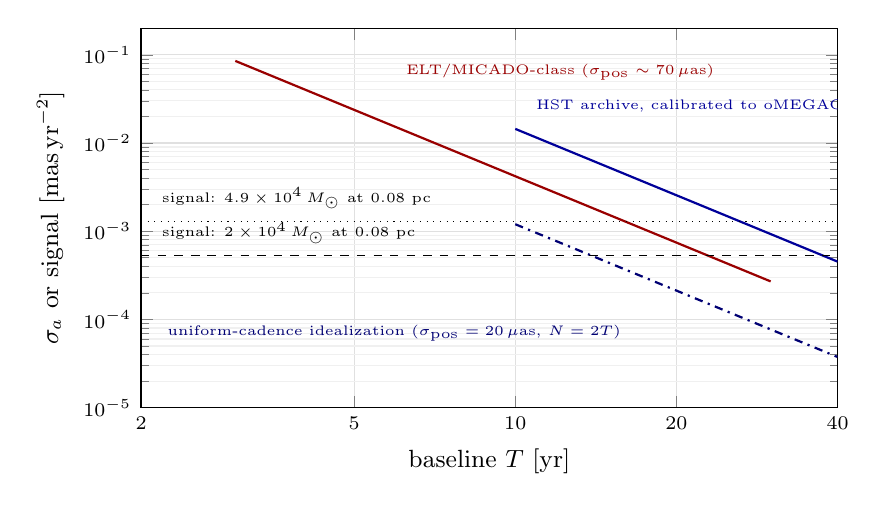
\begin{tikzpicture}
\begin{axis}[
  width=0.86\linewidth, height=6.4cm,
  xlabel={baseline $T$ [yr]}, ylabel={$\sigma_{a}$ or signal [mas\,yr$^{-2}$]},
  xmin=2, xmax=40, ymin=1e-5, ymax=2e-1,
  ymode=log, xmode=log,
  xtick={2,5,10,20,40}, xticklabels={2,5,10,20,40},
  grid=both, minor grid style={black!6}, major grid style={black!12},
  tick label style={font=\scriptsize}, label style={font=\small},
]
% HST archive, calibrated: sigma_a = 7.75*sigma_mu/T with the catalogue's own
% central-region sigma_mu = 6.6 muas/yr at T = 20 yr, scaled as T^-2.5.
\addplot[blue!60!black, thick, domain=10:40, samples=60] {2.5559e-3*(20/x)^2.5};
\node[font=\tiny, blue!60!black, anchor=south west] at (axis cs:10.5,1.6e-2) {HST archive, calibrated to oMEGACat $\sigma_{\mu}=6.6\,\mu$as\,yr$^{-1}$};
% The uniform-cadence idealization Draft v2.6 plotted instead: sigma_pos =
% 0.020 mas with N = 2T, twelve times better than the catalogue reports.
\addplot[blue!45!black, thick, dashdotted, domain=10:40, samples=60] {26.83*0.020/(sqrt(2*x)*x^2)};
\node[font=\tiny, blue!45!black, anchor=north west] at (axis cs:2.15,1.1e-4) {uniform-cadence idealization ($\sigma_{\rm pos}=20\,\mu$as, $N=2T$)};
% ELT/MICADO-class: same sqrt(N) chain, sigma_pos = 0.070 mas, N = 2T (2 epochs/yr)
\addplot[red!60!black, thick, domain=3:30, samples=40] {26.83*0.070/(sqrt(2*x)*x^2)};
\node[font=\tiny, red!60!black, anchor=south west] at (axis cs:6,4.0e-2) {ELT/MICADO-class ($\sigma_{\rm pos}\sim70\,\mu$as)};
% signal lines
\addplot[black, dashed, domain=2:40] {5.3e-4};
\node[font=\tiny, anchor=south west] at (axis cs:2.1,5.6e-4) {signal: $2\times10^{4}\,\msun$ at $0.08$ pc};
\addplot[black, dotted, domain=2:40] {1.3e-3};
\node[font=\tiny, anchor=south west] at (axis cs:2.1,1.38e-3) {signal: $4.9\times10^{4}\,\msun$ at $0.08$ pc};
\end{axis}
\end{tikzpicture}\\[6pt]
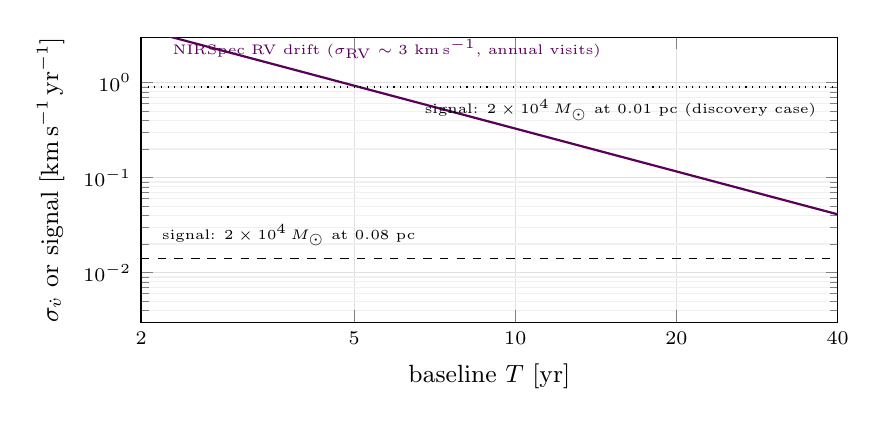
\begin{tikzpicture}
\begin{axis}[
  width=0.86\linewidth, height=5.2cm,
  xlabel={baseline $T$ [yr]}, ylabel={$\sigma_{\dot v}$ or signal [km\,s$^{-1}$\,yr$^{-1}$]},
  xmin=2, xmax=40, ymin=3e-3, ymax=3,
  ymode=log, xmode=log,
  xtick={2,5,10,20,40}, xticklabels={2,5,10,20,40},
  grid=both, minor grid style={black!6}, major grid style={black!12},
  tick label style={font=\scriptsize}, label style={font=\small},
]
% NIRSpec RV drift: sigma = 3*sqrt(12)/(sqrt(T)*T), annual cadence
\addplot[violet!70!black, thick, domain=2:40, samples=40] {10.39/x^1.5};
\node[font=\tiny, violet!70!black, anchor=south west] at (axis cs:2.2,1.4) {NIRSpec RV drift ($\sigma_{\rm RV}\sim3$ km\,s$^{-1}$, annual visits)};
\addplot[black, dashed, domain=2:40] {0.014};
\node[font=\tiny, anchor=south west] at (axis cs:2.1,0.015) {signal: $2\times10^{4}\,\msun$ at $0.08$ pc};
\addplot[black, dotted, domain=2:40] {0.9};
\node[font=\tiny, anchor=north west] at (axis cs:6.5,0.85) {signal: $2\times10^{4}\,\msun$ at $0.01$ pc (discovery case)};
\end{axis}
\end{tikzpicture}
\caption{Why direct acceleration detection on the known fast stars is marginal. \emph{Upper panel:} $1\sigma$ acceleration uncertainty versus baseline, against the expected signals (horizontal lines, Eq.~\ref{eq:accel}). All three curves are the one least-squares chain of Eq.~(\ref{eq:astromchain}). The solid blue curve is the HST archive calibrated through $\sigma_a = 7.75\,\sigma_{\mu}/T$ to the proper-motion precision oMEGACat itself reports inside $r<1.5'$ ($\sigma_{\mu} = 6.6\,\mu$as\,yr$^{-1}$ at $T=20$~yr, scaled as $T^{-2.5}$); the survey-median $\sigma_{\mu} = 11\,\mu$as\,yr$^{-1}$ lies a factor 1.67 above it and is not drawn. The dash-dotted curve is the uniform-cadence idealization plotted in Draft v2.6 ($\sigma_{\rm pos} = 20\,\mu$as with $N = 2T$), retained here as the bracket it is: Eq.~(\ref{eq:astromchain}) makes it equivalent to $\sigma_{\mu} = 0.55\,\mu$as\,yr$^{-1}$, twelve times better than the catalogue delivers, and its apparent $5\sigma$ crossings at $\sim$18~yr (heavy mass) and $\sim$26~yr (nominal) are properties of that assumed cadence rather than of the data. The calibrated curve crosses $5\sigma$ at $\sim$50~yr on the heavy \citet{GonzalezPrieto2025} mass and $\sim$70~yr on the nominal mass, both beyond the plotted range, and crosses $1\sigma$ on the nominal mass at $\sim$38~yr. The red ELT/MICADO curve is a forward forecast at $\sigma_{\rm pos} = 70\,\mu$as and $N = 2T$, with no catalogue to calibrate against; it crosses $5\sigma$ on the heavy mass at $\sim$30~yr and does not reach $5\sigma$ on the nominal mass within the plotted baseline. \emph{Lower panel:} the radial-velocity-drift channel opened by GO 5137-class NIRSpec monitoring (Section~\ref{sec:honest}): at the nominal fast-star radius the verdict matches the proper-motion channel, while an inner star at 0.01~pc crosses the sensitivity curve within a few years. The astrometric program is therefore built around wander, reference-frame, and discovery measurements instead (Section~\ref{sec:wander}).}
\label{fig:astromsens}
\end{figure}

\subsection{Three astrometric measurements}
\label{sec:wander}

\textbf{(i) Photocentric wander (Roman).} An IMBH of mass $M_{\bullet}$ in dynamical equilibrium with a stellar bath executes Brownian motion with velocity $\sigma_{\bullet} \sim \sigma_{*}\sqrt{m_{\rm eff}/M_{\bullet}}$ relative to the cluster centre of mass. The effective mass is the mass-weighted mean $m_{\rm eff} = \langle m^{2}\rangle/\langle m\rangle$, not the number-weighted $\bar m$, because the velocity diffusion scales with $n\langle m^{2}\rangle$ while the drag scales with $n\langle m\rangle$ \citep{ChatterjeeHernquistLoeb2002,MerrittBerczikLaun2007}. The distinction is worth a factor of a few here and it runs in the program's favour: for the segregated mass function adopted in Paper E, $m_{\rm eff} \simeq 2.3\,\msun$ against $\langle m\rangle = 0.54\,\msun$, so the amplitude is $\sim$2.7$\times$ larger than an equal-mass estimate at $\bar m = 0.3\,\msun$ gives, $\sim$13~$\mu$as\,yr$^{-1}$ rather than $\sim$5 at $8{,}200\,\msun$. The lighter the hole, the larger its wander: the predicted amplitude differs by $\sim$17 per cent between $6{,}000$ and $8{,}200\,\msun$ (the square root of the mass ratio), and by a factor $\sim$2.4 between $8{,}200$ and $4.9\times10^{4}\,\msun$. Those ratios are independent of $m_{\rm eff}$, so the pre-registered deliverable below is unaffected by the correction; only the detectability margin moves. Resolving it requires measuring the reflex motion of the innermost stellar distribution at the few-$\mu$as\,yr$^{-1}$ level against the bulk cluster frame: the regime of Roman's wide-field astrometry, which delivers $\sim$10~$\mu$as-class differential astrometry over fields vastly larger than HST's, tying the inner arcseconds to thousands of cluster reference stars at once \citep{Sanderson2019}. Two saturation caveats bound the reference-star pool: \ocen's brightest giants saturate Roman's detectors even in the shortest exposure modes, and the faint end is photon-starved in crowding, so we take the usable reference-star window to be roughly F146 $\approx$ 16--21~mag (a stated assumption to be verified against the as-flown detector performance; the $\gtrsim 10^{3}$ stars-per-field figure below already assumes it). With launch announced for 2026 August 30, a five-year cadenced guest-observer program ($\omega$~Cen lies outside the core community surveys, so epochs must be requested, but the per-epoch cost is small) delivers, as its headline result, the factor-2.4 discrimination between the light-IMBH and heavy-IMBH wander regimes, independently of individual-star orbits. The 17 per cent split inside the light regime is not a deliverable at any plausible reference-frame precision, and Draft v2.6's claim that it would support ``3--5$\sigma$ discrimination'' is withdrawn here. The obstacle is degrees of freedom rather than photon noise. Wander is a variance, so what a campaign measures is the rms of a stochastic amplitude, and the relative error of a variance estimate on $N_{\rm dof}$ independent samples is $\sqrt{2/N_{\rm dof}}$. A 17 per cent amplitude ratio is a 37 per cent variance contrast, so resolving it needs $N_{\rm dof} > 2n_{\sigma}^{2}/0.367^{2}$, which is 134 independent samples at $3\sigma$ and 372 at $5\sigma$. A five-year cadenced program delivering $\gtrsim$10 epochs measures the wander variance to about 45 per cent, four times the contrast it would have to resolve, and averaging over $\gtrsim 10^{3}$ reference stars sharpens the frame tie at each epoch without adding independent samples of the hole's own orbit. The factor-2.4 light-versus-heavy separation asks for $N_{\rm dof} > 1$ at $3\sigma$ and $> 2$ at $5\sigma$ on the same arithmetic, which $\gtrsim$10 epochs meets, and it is the only wander deliverable we pre-register.

That deliverable now carries a numeric pre-condition rather than a promise to quantify one later. The light and heavy predictions are separated by $13.5 - 5.5 = 8.0\,\mu$as\,yr$^{-1}$ at $m_{\rm eff} = 2.3\,\msun$, so a $3\sigma$ separation requires every error combined, $N$-body modelling of the stellar background included, to stay below $2.7\,\mu$as\,yr$^{-1}$ ($1.6\,\mu$as\,yr$^{-1}$ at $5\sigma$). Before the pre-registration locks, the wander prediction will be pushed through the \citet{GonzalezPrieto2025} $N$-body realizations and the model-to-model scatter quoted as the systematic floor; if that scatter exceeds $2.7\,\mu$as\,yr$^{-1}$ the wander channel carries no D2 weight, and Table~\ref{tab:thresholds}'s astrometric row states the condition explicitly alongside the gate on Roman's as-flown crowded-field performance (which has never been measured on a field like this) and the F146 reference-window assumption above.

One error budget the wander calculation implies has been missing from the search geometry. The same Brownian equilibrium that gives the hole a velocity $\sigma_{\bullet}$ gives it a displacement: in the cluster's harmonic core ($\rho_{0} \simeq 3\times10^{3}\,\msun$\,pc$^{-3}$, so $\omega = \sqrt{4\pi G\rho_{0}/3} = 7.35$~km\,s$^{-1}$\,pc$^{-1}$) the one-dimensional rms offset is $r_{\bullet} = \sigma_{\bullet}/\omega$, which at $m_{\rm eff} = 2.3\,\msun$ is $0.048$~pc ($1.80''$) at $8{,}200\,\msun$, $0.056$~pc ($2.10''$) at $6{,}000\,\msun$, and $0.020$~pc ($0.74''$) at $4.9\times10^{4}\,\msun$; the projected two-dimensional rms is $\sqrt{2}$ larger, $2.54''$, $2.97''$ and $1.04''$ respectively. In the light-mass hypotheses this equals or exceeds the $\pm1''$ kinematic-centre uncertainty of Table~\ref{tab:ocparams} and fills the $3''$ fast-star region, so a fixed centre is an assumption the light hypotheses do not license. The rest of the paper carries the consequences. The centre uncertainty used in any search is inflated to $\max(1'', r_{\bullet}(M_{\bullet}))$, which is $2$--$3''$ in the light case. The pointing tolerance for Program 8's ``at the kinematic centre'' trigger and for the X-ray re-registration of Section~\ref{sec:archival} is set the same way. The quoted fast-star radii are wander-smeared at $6$--$8\times10^{3}\,\msun$, which loosens rather than tightens the $r < 3''$ membership. The amplitudes and the required-scatter figure are recomputed in \texttt{paper/figs/fC\_r9\_checks.py}.

The astrometric channel itself now carries a proof of capability: \citet{Whitaker2026BH2} used the same HST astrometric archive (2002--2023), extended with JWST imaging, to detect the reflex wobble of a main-sequence star orbiting an unseen $4.46^{+1.22}_{-1.01}\,\msun$ companion, the first stellar-mass black hole confirmed in \ocen{} and the first astrometric black-hole detection in any globular cluster. A dynamically measured dark remnant in the same field, with a 94-yr period and 31-AU separation recovered from curvature over a two-decade baseline, demonstrates end-to-end that the catalogue's astrometry supports orbit-grade inference at the precision this program assumes.

\textbf{(ii) The absolute reference frame (Gaia DR4, 2026 December).} The dominant systematic in all current inner-field astrometry is the tie between HST's relative frame and the absolute (ICRS) frame. Gaia DR4's 5.5-year solutions for the $r > 10''$ cluster members \citep{GaiaMission2016} improve proper motions by several-fold over DR2-era ties, propagating directly into the fast-star velocity vectors --- and thus into the $8{,}200\,\msun$ lower bound itself, which rests on those velocities exceeding the escape speed. This is the cheapest decisive measurement in the entire campaign: a re-derivation of the \citet{Haberle2024Nature} bound on the DR4 frame either firms the tension into a $>5\sigma$ contradiction with the timing bound or dissolves it. Deliverable in 2027 from archival data alone.

\textbf{(iii) Inner-star discovery (ELT/MICADO, 2029+).} MICADO's $\sim$10~mas resolution and 39-m aperture \citep{Davies2021} penetrate the central arcsecond at magnitudes HST cannot reach in crowding, with the realistic prize being new fast stars at $r < 0.02$~pc. A single star at $0.01$~pc raises the acceleration signal of Eq.~(\ref{eq:accel}) by a factor of 64, converting Figure~\ref{fig:astromsens}'s verdict from ``decades'' to ``a few epochs'' --- this is how the Galactic-Centre program succeeded \citep{GRAVITY2018}, and \ocen{} is its natural successor target at $10^{2}\times$ lower mass. With ELT first light scheduled for 2029 and commissioning occupying the first year of operations, the first MICADO astrometric epochs realistically arrive in 2030--31, at two epochs per year thereafter; first acceleration-grade results by the early 2030s.

\subsection{Decision criteria}

The D1 sample and centre are fixed here, before DR4 lands, because a bound re-derived on a re-chosen sample cannot adjudicate anything. The primary D1 statistic is computed on the five robust fast stars of \citet{Haberle2024Nature}, with the seven-star set (the five plus the two carried as that paper's sensitivity row) reported alongside as a sensitivity check and not as the headline; Table~\ref{tab:mass} labels the sample each bound rests on, since the monitored set and the set the bound is computed from are not the same seven. The centre is the published kinematic centre propagated to the DR4 epoch, not re-fitted to the fast stars themselves, and the aperture is the wander-inflated $\max(1'', r_{\bullet})$ of Section~\ref{sec:wander}. DR4 re-derivation (2027): if the fast-star velocity excess survives at $>5\sigma$ on the five-star sample, $H_1$ requires the MSP analysis to be systematically biased, a specific and checkable claim (radial distribution priors; \citealt{BanaresHernandez2025}). Roman wander (2031): light/heavy discrimination feeds the LISA prior. MICADO inner stars (2030s): any star with measured Keplerian curvature yields $M_{\bullet}$ to tens of per cent, independent of statistical modelling, before LISA flies.

% =====================================================================
\section{Program 4: The LISA forecast}
\label{sec:lisa}

\paragraph{Bottom line.} The decisive observable is an extreme- or intermediate-mass-ratio inspiral caught in band, which would measure the central object's mass and spin regardless of its electromagnetic state. There is no current limit to state; the program is a forecast. The target precision is fractional mass to $10^{-3}$--$10^{-4}$ and spin to $10^{-3}$. Whether it is ever delivered is governed by two probabilities that differ by an order of magnitude or more, so both are quoted. The chance of a new capture during a four-year mission at the \citet{GonzalezPrieto2025} rate is $\sim3\times10^{-7}$; the chance that a compact object is already in band, which is what LISA would actually see, is the residence-weighted occupancy, $\sim2\times10^{-6}$ at 2~mHz rising to $\sim3\times10^{-5}$ at 0.8~mHz for the $31\,\msun$ companion. The occupancy is the decision-relevant number and is what D4 is scored against. A Tier-3 measurement adjudicates the managed-system hypothesis in the same instant it settles the mass tension, and the probable deliverable is the Tier-1 resolved-source count rather than an inspiral.

\subsection{Science case}

LISA is the campaign's final stage: the only instrument that can measure the central object's mass and spin to high precision regardless of its electromagnetic state \citep{Colpi2024,AmaroSeoane2017}. For a compact object inspiralling into a $10^{4}$-class IMBH, matched-filter parameter estimation delivers fractional precisions of order $10^{-3}$--$10^{-4}$ on mass and $10^{-3}$ on spin \citep{Babak2017,AmaroSeoane2018}, a deliberately conservative floor: \citet{Babak2017} reports fractional mass errors as tight as $10^{-6}$ for favourable configurations, and we quote the weaker end of their range throughout. At 5.49~kpc (versus the Gpc distances over which LISA expects to detect its EMRI population), any \ocen{} inspiral in band during the mission would be loud, with matched-filter SNR of order $10^{4}$--$10^{5}$ depending on companion mass (Section~\ref{sec:lisa}), making occurrence probability, not sensitivity, the limiting factor.

\subsection{Occurrence rates}

Event-rate estimates in the LISA literature imply IMRI formation rates per cluster of order $10^{-9}$--$10^{-6}$~yr$^{-1}$ depending on IMBH mass, binary fraction, and core density \citep{Mandel2008,AmaroSeoane2018,Fragione2018,ArcaSedda2021}. A target-specific value is now available and is three decades narrower: the \ocen{} models of \citet{GonzalezPrieto2025}, in which the IMBH grows chiefly by capturing $30$--$40\,\msun$ black holes (mean $31\,\msun$), give a present-day capture rate of $(4$--$8)\times10^{-8}$~yr$^{-1}$. We adopt that figure, and the $31\,\msun$ companion it describes, where a single number is needed, and retain the generic range and its lighter $1.4\,\msun$ companion case as the class-level comparison; the two populations are not interchangeable, and pairing one rate with the other's waveform misstates occurrence by more than an order of magnitude, as the Tier-2 calculation below shows explicitly. Over a 4--10-year mission the generic range yields an in-band inspiral probability for \ocen{} of $\lesssim 10^{-5}$, and the target-specific rate gives $\sim 3\times10^{-7}$ over four years: possibly enhanced by the cluster's unusually dense remnant population, but not by the four to five orders of magnitude required to make it likely.

The forecast is stated in three tiers. \textbf{Tier 1 (probable, no \ocen{} source):} the deliverable is a resolved-source count, not a stochastic-foreground limit. \ocen{} at 5.49~kpc, localized to a $\sim10$-arcmin core, places any in-band binary of the remnant population among LISA's individually resolved sources rather than folded into an unresolved galactic-confusion background; the deliverable this tier owes is a predicted count under $H_0$ and $H_1$ against the observed null, a stronger and more localized test of the extended-component density profile than a foreground amplitude would be. \textbf{Tier 2 (early-inspiral capture):} a compact object caught in the early, slowly evolving portion of an inspiral, in band for years to millennia before plunge depending on companion mass. This is not a distinct source class from Tier 3; it is the same inspiral intercepted earlier, and its detectability and occurrence pull in opposite directions, and both depend on which population is doing the inspiraling. For the target-specific $31\,\msun$ companion the \citet{GonzalezPrieto2025} rate is licensed for: $\mathcal{M}_{c} = 411.9\,\msun$, giving $\dot f = (96/5)\,\pi^{8/3}(G\mathcal{M}_c/c^3)^{5/3}f^{11/3} \approx 1.65\times10^{-12}$~Hz\,s$^{-1}$ at $f_{\rm GW}=2$~mHz, residence $f/\dot f \approx 38$~yr, and a target-specific Tier-2 occupancy $(4$--$8)\times10^{-8}\,{\rm yr^{-1}} \times 38\,{\rm yr} \approx 2\times10^{-6}$; at $0.8$~mHz the residence lengthens to $\approx 440$~yr and the occupancy recovers to $\approx 3\times10^{-5}$. Detectability is overwhelming at either frequency, SNR of order $10^{6}$ over a 4-yr mission against LISA's instrument-only $\sqrt{S_{n}} \approx 3\times10^{-20}$~Hz$^{-1/2}$ at 2~mHz. For the lighter $1.4\,\msun$ companion the generic class-level rate applies, not the target-specific one: $\mathcal{M}_{c}=64.3\,\msun$, $h \approx 3.5\times10^{-19}$ at 2~mHz (orbital radius $\approx 0.03$~AU, $\sim 10^{2}\,r_{g}$) and 5.49~kpc, residence $\approx 850$~yr ($\approx 10^{4}$~yr at 0.8~mHz), SNR of order $10^{5}$ over 4~yr against the instrument floor (even a $0.1\,\msun$ companion accumulates $\sim 7\times10^{3}$), and an occupancy $(10^{-9}$--$10^{-6}\,{\rm yr^{-1}}) \times (10^{3}$--$10^{4}\,{\rm yr}) \approx 10^{-6}$--$10^{-2}$, derived from, not independent of, the Tier-3 rate. That $1.4\,\msun$ range is the generic-rate case, not one \citet{GonzalezPrieto2025} licenses a target-specific rate for; quote the band with both the number and the companion mass. The instrument-only $\sqrt{S_{n}} \approx 3\times10^{-20}$~Hz$^{-1/2}$ used above omits the galactic-confusion foreground, which for a 4-yr mission \citep{Robson2019} adds $78$~per~cent in power at 2~mHz ($\sqrt{S_{n}} \approx 4.0\times10^{-20}$, SNR still of order $10^{5}$ for the $1.4\,\msun$ case) and dominates by a factor $3.4$ at 0.8~mHz ($\sqrt{S_{n}} \approx 4.3\times10^{-19}$), so the low-frequency end of the occupancy range above is bought at a sensitivity cost the raw residence numbers do not price. If any compact object is in band LISA cannot miss it, and the orbital frequency and its drift then measure $M_{\bullet}$ to precision intermediate between timing and a full late inspiral; but the expectation remains that the band is empty. \textbf{Tier 3 (lucky):} a genuine inspiral; per-mille mass and spin. Even in Tier 1, a spin constraint for the class arrives statistically: LISA's detected population of comparable IMBH systems at cosmological distances calibrates the natural spin distribution against which any eventual \ocen{} measurement is judged. The campaign's structure ensures that even Tier 1 is decisive when combined with the pulsar acceleration map (Section~\ref{sec:radio}): a resolved-source non-detection plus a point-mass timing profile isolates $H_0$. \textbf{Tier 4 ($H_1$'s own mHz signature):} a fourth outcome belongs on this tier list even though it never activates $H_2$: a remnant subcluster dense enough to explain $H_1$ contains a substantial stellar-mass black-hole population, and that population produces its own resolvable mHz binaries (SNR $\sim$ few$\times10^{4}$ at 2~mHz over a 4-yr mission), a distinct and unambiguous LISA signature that a null central massive object does not otherwise predict.

\subsection{The spin measurement as the $H_2$ adjudicator}

Paper A dependence (labelled): under $H_2$ the single sharpest residue is near-extremal spin ($\astar \gtrsim 0.9$) on a hole that has demonstrably accreted nothing for Gyr; under $H_0$ natural formation channels for cluster IMBHs span low-to-moderate spin, and for \ocen{} specifically the growth history modelled by \citet{GonzalezPrieto2025} ($\sim$$10^{3}$ captures of $30$--$40\,\msun$ black holes onto a $500$--$5000\,\msun$ seed, seed-epoch mass ratio $q \simeq 0.006$--$0.08$, final-mass ratio $\mu/M_f \simeq 7\times10^{-4}$) is the isotropic minor-merger regime, which under isotropic capture ($\langle\cos\iota\rangle = 0$ for the captured objects) random-walks the spin to $\astar \sim 0.05$--$0.10$ (central $\approx 0.06$; \citealt{Swanson2026Engineered}) rather than toward the $\chi \simeq 0.7$ attractor of comparable-mass hierarchical growth, which the random walk alone reaches only at $q \approx 0.12$, a factor $\sim 175$ above \ocen's final-mass ratio. That prediction holds only while the net-alignment fraction of the captured population stays below $\epsilon_{\rm rot} \approx 0.035$; above it a coherent, unsuppressed spin-up term takes over and the low-spin prediction degrades, a premise \citet{Swanson2026Engineered} states explicitly and recommends checking directly against the \citet{GonzalezPrieto2025} realizations. The contrast this test resolves is therefore the full low-versus-high one at this target, sharper than an earlier draft's $\simeq0.7$-versus-$\gtrsim0.9$ reading; the attractor caveat applies to the class-level LISA population, not to \ocen{}. A Tier 3 spin measurement therefore adjudicates $H_2$ at the same instant it completes the $H_0$/$H_1$ question, the entire reason this campaign's electromagnetic and dynamical groundwork must precede LISA rather than follow it. The full decision tree, including this branch and its isotropy premise, is assembled in Section~\ref{sec:decision}.

\subsection{Deliverables before launch}

Between now and the mid-2030s the program's work is preparatory but concrete: (i) maintain the dynamical model of the inner parsec (timing + astrometry) so that any LISA source has an immediate host context; (ii) publish the \ocen-specific EMRI/IMRI rate forecast with the post-2026 mass constraints folded in; (iii) ensure the cluster's barycentric ephemeris and distance ($\pm$0.06~kpc; \citealt{Haberle2025oMEGACatVI}) are maintained at the precision LISA parameter estimation will assume.

% =====================================================================
\section{Program 5: KM3NeT/ARCA neutrino monitoring}
\label{sec:neutrino}

\paragraph{Bottom line.} The decisive observable is a high-energy neutrino multiplet: at least three tracks within $1^{\circ}$ of the cluster, $E \gtrsim 10$~TeV, inside one sliding window, significant beyond $5\sigma$ post-trials with no astrophysical counterpart. The current best is the archival ANTARES+IceCube baseline, with ARCA at 51 of 230 detection units and sensitivity growing roughly linearly through the decade. The target is full-array steady-state point-source sensitivity of a few $\times10^{-12}$--$10^{-11}$~TeV~cm$^{-2}$~s$^{-1}$ plus a decade-scale burst pipeline over $\sim3\times10^{6}$ windows. A null closes the burst-mode channel at its stated strength; any candidate triggers the two-messenger protocol of Section~\ref{sec:coordination}.

\subsection{Science case and geometry}

\ocen{} at declination $-47.5^{\circ}$ is an up-going source for the Mediterranean: KM3NeT/ARCA observes it through the Earth, with atmospheric muons filtered out and sub-$0.2^{\circ}$ angular resolution for track events at $\gtrsim$10~TeV \citep{AdrianMartinez2016}. For IceCube the same source is down-going (degraded but usable above $\sim$100~TeV; \citealt{IceCubePS2020}); the combined ANTARES+IceCube southern-sky analysis \citep{AntaresIceCube2020} defines the archival baseline. ARCA stood at 51 of 230 detection units as of early 2026, with real-time alert distribution entering commissioning; sensitivity grows roughly linearly with instrumented volume through the decade. The partially built array has already delivered a discovery-class result: the $\sim$220-PeV track event KM3-230213A, the most energetic neutrino yet observed \citep{KM3NeT2025}, demonstrates that ARCA detects and reconstructs the rare high-energy events on which this program's burst criterion rests. The conventional science driver is a deep point-source limit on a dense old stellar system; the technosignature driver (Paper A dependence, labelled) is the burst-mode prediction of black-hole-based computation models \citep{Dvali2023,Lacki2025}, for which a cluster like \ocen{} is the natural test bed and which the existing point-source pipelines do not target: their time-integrated statistics dilute rare short multiplets.

\subsection{Implementation}

\textbf{Steady-state search (archival + ongoing).} Standard unbinned-likelihood point-source analysis \citep{Braun2008} at the \ocen{} coordinates in (i) the ANTARES+IceCube combined dataset, (ii) the growing ARCA exposure. Full-array ARCA reaches $E^{2}\Phi \sim$ few~$\times10^{-12}$--$10^{-11}$~TeV\,cm$^{-2}$\,s$^{-1}$ at this declination over multi-year integrations --- the deepest neutrino limit ever placed on a globular cluster.

\textbf{Burst pipeline (new, the campaign's contribution).} A pre-registered transient search in windows of $10^{2}$, $10^{3}$, and $10^{4}$~s within $1^{\circ}$ of the cluster centre, $E \gtrsim 10$~TeV, on ARCA data plus IceCube alerts. The background expectation calibrating the criterion is an atmospheric-neutrino rate above 10~TeV within a $1^{\circ}$ cone of $10^{-7}$~s$^{-1}$ ($\sim$3 events\,yr$^{-1}$ in the cone), a deliberate $\sim$20$\times$ envelope on the $\sim$0.15~yr$^{-1}$ that Paper A derives for the same cone from the KM3NeT 2.0 letter of intent \citep{AdrianMartinez2016}, as inherited via \citealt{Swanson2026MTH}, and one that likely overstates the measured up-going rate for a cone this size by one to two orders of magnitude.

The trials budget is window-dependent, and so is the criterion. A decade of monitoring holds $3.16\times10^{6}$ non-overlapping $10^{2}$-s windows, $3.16\times10^{5}$ at $10^{3}$~s and $3.16\times10^{4}$ at $10^{4}$~s, so a single trials count cannot serve all three. Under the $20\times$ envelope a triplet gives post-trials false alarms of $5.3\times10^{-10}$ ($6.1\sigma$) at $10^{2}$~s and $5.3\times10^{-8}$ ($5.3\sigma$) at $10^{3}$~s, both clearing the $5\times10^{-7}$ action boundary, and $5.3\times10^{-6}$ ($4.4\sigma$) at $10^{4}$~s, which does not. The pre-registered criterion is therefore $\geq 3$ tracks at $10^{2}$ and $10^{3}$~s and $\geq 4$ tracks at $10^{4}$~s, the last giving $1.3\times10^{-9}$ ($6.0\sigma$); under the realistic $4.75\times10^{-9}$~s$^{-1}$ rate a triplet clears $5\sigma$ at all three window sizes, so the raised multiplicity costs nothing except in the envelope case it is there to cover. Draft v2.6's ``$\sim 5\times10^{-7}$ ($\approx 5\sigma$)'' is withdrawn: it pairs the $10^{3}$-s expectation with the $10^{2}$-s window count, a combination that reproduces $5.3\times10^{-7}$ and belongs to no single window size. Windows are treated as non-overlapping for the trials count; a sliding search at finer step inflates the count by the oversampling factor and must be priced at analysis time. The recomputation is in \texttt{paper/figs/fC\_r9\_checks.py}. Any KM3NeT or IceCube real-time alert within $1^{\circ}$ triggers the electromagnetic protocol of Section~\ref{sec:coordination}, and the alert system's first \ocen-relevant cycle begins in late 2026.

\begin{figure}[tbp]
\centering
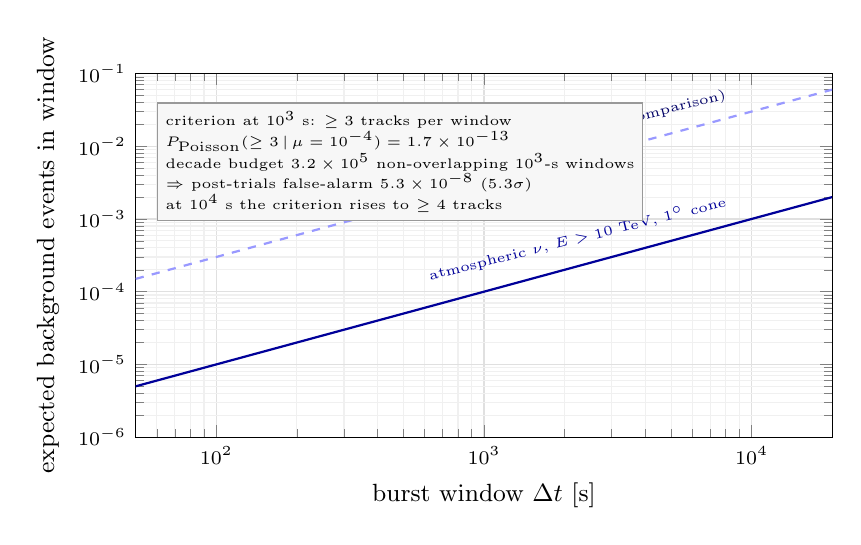
\begin{tikzpicture}
\begin{axis}[
  width=0.86\linewidth, height=6.2cm,
  xlabel={burst window $\Delta t$ [s]}, ylabel={expected background events in window},
  xmode=log, ymode=log,
  xmin=50, xmax=2e4, ymin=1e-6, ymax=1e-1,
  grid=both, minor grid style={black!6}, major grid style={black!12},
  tick label style={font=\scriptsize}, label style={font=\small},
]
% atm nu background: 1e-7/s * dt
\addplot[blue!60!black, thick, domain=50:2e4, samples=2] {1e-7*x};
\node[font=\tiny, blue!60!black, anchor=south east, rotate=14] at (axis cs:9e3,1.1e-3) {atmospheric $\nu$, $E>10$ TeV, $1^{\circ}$ cone};
% atm nu at 1 TeV threshold for comparison: ~3e-6/s
\addplot[blue!40, thick, dashed, domain=50:2e4, samples=2] {3e-6*x};
\node[font=\tiny, blue!40!black, anchor=south east, rotate=14] at (axis cs:9e3,3.2e-2) {same, $E>1$ TeV (for comparison)};
% Poisson P(>=3) ~ (mu^3)/6 contour idea: show mu where triplet prob = 1e-9 (5 sigma-ish pre-trials)... instead annotate
\node[font=\tiny, align=left, anchor=north west, draw=black!40, fill=black!3, inner sep=3pt] at (axis cs:60,4e-2)
 {criterion at $10^{3}$~s: $\geq 3$ tracks per window\\
  $P_{\rm Poisson}(\geq 3\,|\,\mu = 10^{-4}) = 1.7\times10^{-13}$\\
  decade budget $3.2\times10^{5}$ non-overlapping $10^{3}$-s windows\\
  $\Rightarrow$ post-trials false-alarm $5.3\times10^{-8}$ ($5.3\sigma$)\\
  at $10^{4}$~s the criterion rises to $\geq 4$ tracks};
\end{axis}
\end{tikzpicture}
\caption{Design of the neutrino burst search. Expected atmospheric-neutrino background within $1^{\circ}$ of $\omega$~Cen versus window length, for the working $E>10$~TeV threshold (solid) and a softer 1~TeV threshold (dashed). At $10^{3}$~s the expectation is $\sim10^{-4}$ events, so the triplet criterion clears $5\sigma$ post-trials at $10^{2}$ and $10^{3}$~s under the $20\times$ envelope; at $10^{4}$~s it reaches only $4.4\sigma$ against that envelope, which is why the pre-registered multiplicity rises to four tracks in the longest window. Rate normalizations are order-of-magnitude, with exact values set by the detector Monte Carlo at analysis time.}
\label{fig:burst}
\end{figure}

The $\geq3$-track multiplet criterion reaches $p_{\rm det} \approx 0.9$ only for burst fluences exceeding an RX-J1713-equivalent steady source by $\sim1.1\times10^{5}$ in a $10^{3}$-s window, and $2.3\times10^{5}$ for $p_{\rm det} \approx 0.999$; the amplification scales inversely with window length, so the same $p_{\rm det}$ needs $10^{6}$ at $10^{2}$~s and $10^{4}$ at $10^{4}$~s (the ARCA effective-area integral, calibrated on the LOI's own event-rate table for the RX J1713 track analysis: 8.1 $\nu_\mu$ tracks in 5 years after final cuts at a source declination of $-39.8^{\circ}$, the same near-horizon visibility class as \ocen{} at $-47.5^{\circ}$). At astrophysically scaled fluences $p_{\rm det} \ll 1$, and the excluded burst rate scales as $1/p_{\rm det}$. The channel is therefore a test of an extraordinary hypothesis, burst fluences that no known astrophysical source produces, rather than a monitor of conventional neutrino emission.

\subsection{Decision criteria}

A decade-scale null at full-array sensitivity closes the burst-mode channel of \citet{Dvali2023} for this system at its predicted strength --- a publishable falsification regardless of $H_2$ (the underlying micro-black-hole physics is itself contested; \citealt{AlvarezDominguez2024,Loeb2024Comment}). One confirmed multiplet with no counterpart, repeated at the same location, would be among the most significant anomalies in high-energy astrophysics independent of any ETI interpretation; the protocol deliberately treats it as an astrophysical discovery first.

% =====================================================================
\section{Program 6: archival Fermi-LAT and CTAO-South gamma rays}
\label{sec:gamma}

\paragraph{Bottom line.} The decisive observable is a Fermi-LAT transient coincident with a Program-5 neutrino window, with a spectral excess above the few-GeV MSP cutoff and a CTAO TeV detection or limit as the conventional-science counterpart. The current best is the H.E.S.S.-era cluster survey limit. The targets are a sliding-window transient search over the full $>$17-year LAT exposure, any emission above $\sim$30~GeV flagged as non-MSP, and a 50-h CTAO-South exposure reaching $\sim10^{-13}$~erg~cm$^{-2}$~s$^{-1}$ at 1~TeV. The program feeds the confirmation tier of the coordination protocol and screens dark-matter-versus-exotica readings before anomaly language.

\subsection{Science case}

\ocen{} is a GeV source: 4FGL J1326.7$-$4729 coincides with the core, and its emission is attributed to the MSP ensemble after deep searches found no individual pulsations \citep{Dai2020,Dai2023}. This is both foreground and opportunity: the steady MSP emission is a calibration source against which \emph{transient} or \emph{spectrally anomalous} excesses can be sought with high contrast. The technosignature channel shares the burst phenomenology of Program 5 (the \citealt{Dvali2023} spectrum is ``democratic'' across species, implying $\gamma$-ray counterparts to any neutrino burst); the conventional channel is a TeV detection or limit on the cluster, of independent interest for MSP magnetospheric and inverse-Compton physics.

\subsection{Implementation}

\textbf{Fermi-LAT (archival, immediate).} Re-analysis of the now $>$17-year LAT exposure at the cluster position: (i) refit of the steady source with current diffuse models; (ii) a sliding-window transient search ($\Delta t = 10^{2}$--$10^{4}$~s, matched to Program 5's windows) over the full mission, with the steady MSP flux as null model; (iii) spectral-cutoff analysis: MSP ensembles cut off at a few GeV, so any significant emission above $\sim$30~GeV flags a non-MSP component. All three are pure archival analyses.

\textbf{CTAO-South (2027+).} The first Paranal telescopes are, on early-2026 construction schedules, arriving through late 2026 \citep{CTAConsortium2019}; intermediate arrays operate while construction proceeds. We propose (i) a 50-h deep exposure reaching $\sim 10^{-13}$~erg\,cm$^{-2}$\,s$^{-1}$ at 1~TeV ($\sim0.2$~per~cent of the Crab Nebula flux at 1~TeV on the HEGRA Crab spectrum, \citealt{Aharonian2000HEGRACrab}) for the completed Alpha-configuration array; the 2027-era partial array delivers a factor 2--4 less, and the depth quoted here is recovered as construction completes. Either figure substantially betters the archival VHE limits placed on globular clusters by the H.E.S.S.\ cluster survey \citep{HESS2013}, making this the first CTAO-depth TeV limit on any globular cluster core. We also propose (ii) a standing target-of-opportunity trigger: any Program-5 alert within $1^{\circ}$ pre-authorizes prompt CTAO follow-up, the latency being minutes for a source that transits Paranal $\sim 23^{\circ}$ from zenith.

\subsection{Decision criteria}

A LAT transient coincident with a neutrino window elevates any Program-5 candidate to the campaign's highest tier. A TeV detection of steady emission is conventional astrophysics: it would make \ocen{} the second globular cluster with detected VHE emission, after H.E.S.S.'s detection coincident with Terzan~5 \citep{Abramowski2011}, and the first with a resolved connection to a candidate IMBH environment. Its absence at CTAO depth tightens the inverse-Compton budget of the MSP population well beyond the existing H.E.S.S.-era cluster limits \citep{HESS2013}. Spectral excess above 30~GeV without transient behaviour prompts a dark-matter-versus-exotica analysis before any $H_2$ language is entertained.

% =====================================================================
\section{Program 7: optical/IR time domain with Rubin/LSST and archival anomalies}
\label{sec:timedomain}

\paragraph{Bottom line.} The decisive observable is a nuclear tidal-disruption event, the one natural signal that would announce the central object unambiguously, together with a population-level photometric anomaly class at $\geq3\sigma$ from the archival census. There is no current detection; the oMEGACat archive is essentially unmined for variability. The targets are an LSST broker filter flagging nuclear transients at $r \gtrsim 16$ and all-sky coverage of the saturated bright regime, plus a variability census of $\sim10^{6}$ stars to $\sim0.05$~mag depth over two decades of baseline. A TDE feeds the pre-arranged multi-wavelength response; anomaly classes feed the coordination protocol.

\subsection{Science case}

Two distinct searches share this program. First, transients: tidal disruption of a star by an IMBH is the one natural event that would announce the central object unambiguously \citep{Hills1988,Gezari2021}; rates are low ($\sim 10^{-7}$--$10^{-6}$~yr$^{-1}$ per cluster for full disruptions, higher for partial-disruption flares of the dense remnant environment) but the cost of monitoring is now effectively zero, because Rubin has taken science data since late 2025 (Pre-LSST), the ten-year LSST formally began on 2026 June 30, and \ocen{} sits in the survey footprint \citep{Ivezic2019}. Second, archival photometric anomalies: the oMEGACat HST archive (500+ epochs over 20+ years for $10^{6}$ stars; \citealt{Haberle2024oMEGACatII,Nitschai2023}) is an essentially unmined time-domain dataset in which periodic dimmings, secular fades, or statistically anomalous variability classes (the photometric residues conjectured for megastructures; \citealt{Wright2014,Hsiao2021,SocasNavarro2021}) can be sought with two decades of baseline for free.

\subsection{Implementation}

\textbf{LSST stream and bright-transient coverage.} At the cluster's distance modulus of $\mu = 13.7$, a full TDE peaking at $M_V \approx -14$ to $-17$ would appear at $V \approx 0$ to $-3$: hopelessly saturated for LSST difference imaging, and indeed for any survey-class imager. The bright-event trigger therefore belongs to ASAS-SN/Evryscope-class all-sky photometry, which monitors this magnitude range continuously; the campaign's role is to register the \ocen{} position with those pipelines. Both instruments saturate well short of the TDE peak: ASAS-SN saturates at $V \approx 10$--11~mag \citep{Kochanek2017}, and Evryscope's short-exposure photometry is saturation-limited near $V \approx 6$~mag \citep{Law2015}, so the bright-transient trigger relies on the recovered, non-linear photometry of saturated frames rather than on standard aperture photometry. LSST covers the complementary faint regime: a standing broker filter on the field flags (i) any nuclear transient in the unsaturated range $r \gtrsim 16$, which captures partial disruptions and other sub-luminous accretion flares, and (ii) anomalous variables among $\sim10^{5}$ measurable members outside the saturated core. Difference-imaging in the crowded annulus is handled with the oMEGACat reference catalogue.

\textbf{Archival mining.} A systematic variability census of the oMEGACat photometric archive: period search to $\sim$0.05~mag depth across $10^{6}$ stars, secular-trend extraction, and an explicitly pre-registered anomaly statistic (population-level excess of non-physical light-curve classes) with human vetting of survivors. Conventional yield: the deepest variable-star census of any globular cluster, eclipsing-binary distance cross-checks, and stellar-rotation demographics --- publishable regardless of anomalies.

\textbf{Core-depletion statistic (joint with Program 3).} Paper A dependence (labelled): $H_2$'s P4c predicts secular depletion of the loosely bound core population beyond $N$-body expectations. The measurement (star counts by binding-energy quantile against matched $N$-body models; \citealt{GonzalezPrieto2025}) is identical to standard mass-segregation analysis and is conventional dynamics on its face; it operationalizes Paper A's P4c observable, stated there as a mass-function-slope test, as a binding-energy-quantile star count instead. We do not pre-register the depletion direction as a primary discriminant: at the 10-pc delivery radius the Phase-4 deficit is $\sim$1 per cent of the enclosed mass, the removed mass reappears as central point mass, and any deficit refills on the $\sim$4-Gyr core relaxation time \citep{Swanson2026Engineered}.

\subsection{Decision criteria}

A nuclear TDE settles the IMBH question electromagnetically (and its decay light curve constrains $M_{\bullet}$; \citealt{Gezari2021}); the campaign's role is to guarantee the multi-wavelength response is pre-arranged. Archival anomalies are population statistics: no single weird star means anything (the false-positive history of photometric SETI is long); only a $\geq 3\sigma$ class-level excess, surviving vetting, enters the coordination protocol.

% =====================================================================
\section{Program 8: Supplementary archival channels}
\label{sec:archival}

\paragraph{Bottom line.} The decisive observable is an X-ray point source at the kinematic centre, at any flux; continuous-wave searches at twice the known pulsar spin frequencies and a stacked ultra-high-energy cosmic-ray directional analysis complete the messenger coverage. The current best is the $\sim$291~ks Chandra limit of $L_{X} \lesssim 1.6\times10^{30}$~erg~s$^{-1}$. The targets are a re-derivation of that limit at the current centre, stacked Chandra/XMM-Newton depth, an eROSITA variability screen, O5-class CW limits of $h_{0} \lesssim 10^{-26}$, and a public-data UHECR stack. The X-ray result feeds the joint fundamental-plane constraint with Programs 1 and 2.

Three channels are cheap enough to run as graduate-student archival projects and complete the messenger coverage.

\textbf{Archival X-rays (Chandra, XMM-Newton, eROSITA).} The X-ray band is the standard probe of quiescent black-hole accretion, and the campaign as presented so far would otherwise lack it. The benchmark limit is the $\sim$291~ks Chandra exposure of \citet{Haggard2013}, which detects no central point source and bounds the unabsorbed luminosity at $L_X(0.5$--$7.0~\mathrm{keV}) \lesssim 1.6\times10^{30}$~erg\,s$^{-1}$, an Eddington ratio of $\lesssim 10^{-12}$ for a $10^{4}\,\msun$ hole. The archival program re-derives this limit at the current oMEGACat kinematic centre (the 2013 analysis predates the fast-star centre determination), searching within the wander-inflated tolerance $\max(1'', r_{\bullet}(M_{\bullet}))$ of Section~\ref{sec:wander} rather than at a fixed position, stacks the subsequent Chandra and XMM-Newton exposures of the field, and folds in the released eROSITA all-sky survey epochs (eRASS1 in the DR1 release, plus the subsequent completed passes as the consortium releases them) as a variability screen, noting that the survey was halted in February 2022, so the eROSITA screen covers 2020--2022 only; a joint X-ray--radio treatment through the fundamental plane \citep{Merloni2003} then constrains radiatively inefficient flow models alongside the Program 1 and Program 2 limits. For reproducibility the re-registration is defined against stated epochs rather than against a position alone: the oMEGACat centre is propagated from its own catalogue reference epoch to the 2013 exposure's epoch using the cluster's absolute proper motion, both epochs are reported with the re-derived limit, and the search aperture is the wander-inflated $\max(1'', r_{\bullet})$ rather than a point. Any X-ray point source at the kinematic centre, at any flux, would be a major result; the expected null sharpens the deepest multi-band quiescence measurement for any black hole candidate.

\textbf{Continuous gravitational waves (LIGO--Virgo--KAGRA).} Narrowband searches at twice the spin frequencies ($f_{\rm GW} = 2f_{\rm spin}$) of the nineteen known MSPs, using public O5 data and the MeerKAT ephemerides, following the known-pulsar methodology of \citet{LVKPulsars2022}. Expected upper limits $h_{0} \lesssim 10^{-26}$ are an O5-class expectation (a factor $\gtrsim2$ better than the best O3 targeted result, PSR~J0711$-$6830, once converted to this frequency band) and translate, at \ocen's own MSP population, which clusters near $P \approx 4$~ms ($f_{\rm GW} \approx 500$~Hz), to ellipticity limits $\varepsilon \approx 2.1\times10^{-7}$ at 5.49~kpc. Reaching a few~$\times10^{-8}$ needs a faster spinner than any known \ocen{} MSP: at $P = 2.5$~ms ($f_{\rm GW} = 800$~Hz) the limit is $\varepsilon \approx 8\times10^{-8}$, and $3\times10^{-8}$ requires $P \approx 1.5$~ms. This is conventional neutron-star physics in an environment (a dense old cluster) where the recycled-pulsar population is dynamically distinctive, with one complication the standard pipeline does not carry: the observed $\dot f$ of a cluster MSP is dominated by line-of-sight acceleration in the cluster potential rather than intrinsic spin-down, several \ocen{} MSPs have measured negative $\dot f$ for exactly this reason, which Program~2's own timing-acceleration map exploits as signal rather than noise. The search must therefore fit $\dot f$ and $\ddot f$ as free terms rather than assume a spin-down model, and the spin-down-limit framing standard targeted searches quote is not available for these targets. The trials factor across the nineteen targets is carried in the post-trials threshold of Table~\ref{tab:thresholds}. The technosignature reading (structured masses in MSP orbits) is not separately funded; it shares the identical data product.

\textbf{Ultra-high-energy cosmic rays (Pierre Auger).} \ocen{} sits well inside Auger's southern acceptance. A stacked directional analysis around the cluster position in the public $E > 8$~EeV dataset \citep{Auger2017}, with $1^{\circ}$ and $3^{\circ}$ apertures bracketing magnetic deflection, either contributes an upper limit on hadronic acceleration in the core (of conventional interest given the MSP wind population) or flags an anisotropy for which the Galactic-Centre region ($52.4^{\circ}$ away, but the dominant anisotropy structure at these energies) is the confounder to exclude first.

% =====================================================================
\section{Coordination, joint statistics, and data policy}
\label{sec:coordination}

\subsection{The two-messenger rule, operationalized}

Table~\ref{tab:thresholds} pre-registers the campaign's trigger and confirmation matrix. Each row names a primary trigger, the channels that can confirm it, and the joint-significance requirement. Combined significances across independent channels use Fisher's method on the per-channel $p$-values; each per-channel $p$-value entering the combination must itself be post-trials within its channel (its look-elsewhere budget over windows, frequencies, and positions already paid), so the combination never launders pre-trials significances. Two opposing effects enter the combined significance; both are stated. Because post-trials $p$-values are conservative rather than uniform under the null, the Fisher combination inherits that conservatism. But Fisher's method assumes the inputs are independent under the null, and several of the pairings in Table~\ref{tab:thresholds} are not: a genuine tidal-disruption flare excites P1, P2, P7 and P8 together, and the LAT and CTAO rows share both the Galactic diffuse model and the cluster's own millisecond-pulsar population. Under positive dependence the Fisher statistic has larger variance than the $\chi^{2}_{2n}$ reference, so the tail probability is understated and the method is anti-conservative. The two effects have no reason to cancel. We therefore apply \citet{Brown1975} for any combination whose inputs are not demonstrably independent under the astrophysical null, estimating the null covariance of the per-channel statistics from archival data (which costs no observing time) and rescaling the degrees of freedom accordingly; the covariance-estimation procedure is pre-registered alongside the thresholds, though the specific archival datasets it will draw on are not yet selected and this element of the plan remains aspirational. Where the covariance is not yet estimated, the combination is restricted to channel pairs that are independent by construction, and the stated global threshold bounds rather than equals the nominal false-alarm rate. The $5\times10^{-7}$ figure is a per-trigger-class threshold, not a campaign-wide false-alarm budget over the ten trigger rows and fifteen years of monitoring; a campaign-wide false-alarm budget aggregating all ten channels is not computed in this paper and is deferred to the individual pipeline papers. The global claim threshold is set at $p < 5\times10^{-7}$ post-trials --- deliberately at discovery convention, because the base rate of true technosignatures is unknown and plausibly zero, so the loss function is asymmetric: a false positive damages the field's credibility far more than a delayed true positive damages the discovery \citep{Wright2022}.

This matrix is one of two pre-registrations governing the campaign, and the two occupy different layers. The Fisher-combined $p < 5\times10^{-7}$ matrix of Table~\ref{tab:thresholds} is the \emph{trigger layer}: it decides when an event or excess is promoted from a single-channel candidate to a campaign-level anomaly requiring adjudication. Paper E's hierarchical Bayes-factor framework, with Kass--Raftery $\ln K$ action bands \citep{Kass1995} whose ``candidate'' band itself requires evidence in at least two messengers, is the \emph{inference layer}: it takes any promoted trigger and adjudicates it against the full $H_q$/$H_{\rm sub}$/$H_{\rm eng}$ hypothesis set \citep{Swanson2026Engineered}. The frequentist matrix therefore controls the false-alarm budget of what enters adjudication, while the Bayesian framework determines what the adjudicated evidence supports; a trigger that clears Table~\ref{tab:thresholds} but lands in a weak $\ln K$ band is reported as an unexplained astrophysical candidate, not an anomaly claim. One mandatory rule governs the interface between the layers. Promotion is data-dependent, so the inference layer always evaluates its likelihoods on the complete campaign record, every epoch and every channel including those that recorded nothing, never on the promoted subset alone. The trigger layer allocates follow-up effort and carries no inferential weight. Scoring only the promoted data would require an explicit selection correction of order $\ln P(\text{trigger}\mid H_0) \approx -14$ nats at the threshold above, which is large enough to move a nominal candidate to null-favoured; carrying the full record avoids the correction rather than paying it \citep{Swanson2026Engineered}. The significance conventions of the two layers, and of the companion papers that consume or produce them, are set side by side in Appendix~\ref{app:conventions}.

\begin{table}[tbp]
\centering
\caption{Pre-registered trigger and confirmation matrix. ``Joint'' = Fisher-combined post-trials significance required for any anomaly claim; single-channel events, however significant, are reported as astrophysical candidates only.}
\label{tab:thresholds}
\scriptsize
\begin{tabular}{p{3.4cm}p{2.6cm}p{3.6cm}p{4.0cm}}
\toprule
Primary trigger & Channel threshold & Confirming channels & Disposition \\
\midrule
Neutrino multiplet (P5) & $\geq 3$ tracks at $10^{2}$--$10^{3}$~s, $\geq 4$ at $10^{4}$~s / $1^{\circ}$ / $\geq$10 TeV, $5\sigma$ post-trials against the $20\times$ background envelope, trials counted per window size & Fermi-LAT window (P6); CTAO ToO (P6); JWST/ground IR (P1) & repeat at same position required for anomaly claim; single event published as astrophysical transient \\
Narrowband radio line (P2) & SNR $>15$; multi-beam cross-rejection; multi-epoch scintillation-aware confirmation (Section~\ref{sec:radio}) & off-source cadence; second telescope (e.g.\ ATCA) & interference exclusion protocol precedes any claim \\
IR variable/transient (P1, P7) & $5\sigma$ on the two-epoch difference ($\geq20$\% amplitude above 118~nJy at NIRCam, above 5.9~$\mu$Jy at F1000W; Section~\ref{sec:jwstexisting}) or new source $>5\sigma$ & radio continuum (P2); X-ray archival; LSST stream (P7) & classified as accretion/TDE candidate first \\
Photometric anomaly class (P7) & $\geq 3\sigma$ population-level excess & independent archive (Gaia epochs); spectroscopy & population statistic only; no single-star claims \\
Astrometric anomaly (P3) & wander outside $H_0$/$H_1$ envelopes at $3\sigma$; light-versus-heavy factor-2.4 separation only, the 17\% within-light-regime split retired on degrees of freedom (Section~\ref{sec:wander}); gated on a measured $N$-body model-to-model scatter below $2.7\,\mu$as\,yr$^{-1}$, on verified Roman crowded-field astrometric performance, and on the F146 $\approx$ 16--21 reference window (core-depletion statistic retired as a primary discriminant: at the 10-pc delivery radius the Phase-4 deficit is $\sim$1 per cent of the enclosed mass, the removed mass reappears as central point mass, and any deficit refills on the $\sim$4-Gyr core relaxation time; \citealt{Harris1996,Swanson2026Engineered}) & timing acceleration map (P2) & feeds LISA prior; no standalone claim \\
$>$30 GeV spectral excess (P6) & $\geq 5\sigma$ non-MSP component in LAT refit & CTAO follow-up (P6); radio/X-ray positional coincidence (P2, P8) & dark-matter-versus-exotica analysis precedes any anomaly language \\
CW detection at MSP frequency (P8) & $\geq 5\sigma$ in known-pulsar narrowband search & EM timing solution and position (P2) & classified as neutron-star physics first \\
UHECR anisotropy (P8) & $\geq 3\sigma$ post-trials stacked excess, $1^{\circ}$--$3^{\circ}$ apertures & Fermi-LAT/CTAO coincidence (P6); Galactic-Centre confounder excluded & directional statistic only; no source claim without $\gamma$-ray support \\
X-ray point source at centre (P8) & any source $>3\sigma$ at kinematic centre & radio continuum (P2); JWST IR counterpart (P1) & classified as accretion candidate; feeds fundamental-plane fit \\
LISA spin/mass result (P4) & per mission parameter estimation & all of the above as context & adjudicates $H_0$/$H_1$/$H_2$ per Section~\ref{sec:decision} \\
\bottomrule
\end{tabular}
\end{table}

\subsection{Alert latency and standing authorizations}

The latency-critical path is neutrino $\rightarrow$ gamma/optical: KM3NeT real-time alerts (commissioning through 2026) distribute within seconds--minutes; the CTAO ToO and LSST-broker hooks are standing authorizations requiring no human decision for the first response hour. Slow-path coordination (JWST DDT requests, radio re-pointing) is pre-drafted as template proposals with trigger criteria attached, cutting submission latency to $<$24~h.

\subsection{Data policy}

All pipelines, thresholds, and analysis code are public from the start (the pre-registration is itself the methods paper); all derived catalogues are released with their papers; raw data inherit host-facility policies. That guarantee covers what the campaign controls: its own code, thresholds, and derived products. What host collaborations must grant is a separate matter, negotiated by memorandum of understanding and costed in Table~\ref{tab:cost}: MeerKAT and SKA raw data fall under SARAO proprietary policy, and KM3NeT does not release track-level data outside the collaboration, so the Program-5 burst pipeline runs either inside the collaboration on the full stream or externally on the much smaller public alert stream. Negative results are published on a fixed, pre-announced cadence, so that the decision to publish never depends on what the data showed.

\subsection{Program summary}

Table~\ref{tab:programs} assembles the eight programs with sensitivities, requests, and timelines.

\begin{table}[tbp]
\centering
\caption{Campaign summary. ``Type'': A = archival/commensal, N = new observations, F = free by-product of funded survey. Costs are rough full-cost estimates (Section~\ref{sec:cost}); facility time is listed separately since it is allocated, not purchased.}
\label{tab:programs}
\scriptsize
\begin{tabular}{p{0.45cm}p{2.5cm}p{0.5cm}p{3.6cm}p{2.5cm}p{1.6cm}p{2.2cm}}
\toprule
\# & Program & Type & Key sensitivity & Facility request & Timeline & Decides \\
\midrule
P1 & JWST IR limits & N & $\sim$10 nJy (F444W); $L_{\rm bol} \lesssim 10^{30}$ erg s$^{-1}$ & $\sim$65 h, 2 epochs & 2027--2029 & accretion state; waste heat \\
P2 & Radio: timing + SETI + continuum & N & $\sigma_a \sim 10^{-10}$ m s$^{-2}$ (5 yr); EIRP $4\times10^{15}$ W (incoh., full cluster) & $\sim$130 h yr$^{-1}$ MeerKAT, 5 yr & 2026--2031+ $\to$ SKA-Mid & $H_0$ vs $H_1$ (profile); first SETI limit \\
P3 & Astrometry: DR4 + Roman + ELT & A/F/N & frame to DR4; wander factor-2.4 (light vs heavy); inner-star discovery & archival; Roman survey; $\sim$28 h ELT (dedicated) & 2026--2035 & mass tension; wander mass \\
P4 & LISA forecast & F & $\delta M/M \sim 10^{-3\text{--}4}$, $\delta\astar \sim 10^{-3}$ (if inspiral) & none (mission science) & 2035+ & everything (Tier 3) \\
P5 & Neutrino monitoring & A/N & $E^{2}\Phi \sim$ few$\times10^{-12}$ TeV cm$^{-2}$ s$^{-1}$; burst triplets & pipeline on ARCA stream & 2026--2040 & Dvali--Osmanov channel \\
P6 & Gamma rays & A/N & LAT transient windows; $10^{-13}$ erg cm$^{-2}$ s$^{-1}$ at 1 TeV (50 h) & 50 h CTAO + ToO & 2026--2032 & burst counterparts; first CTAO-depth TeV limit \\
P7 & Time domain & A/F & TDE flares unmissable; $10^{6}$-star archival census & LSST stream; archival & 2026--2036 & TDE; anomaly classes \\
P8 & X-ray + CW + UHECR archival & A & $L_X \lesssim 10^{30}$ erg s$^{-1}$; $h_0 \lesssim 10^{-26}$; stacked UHECR limit & public data & 2026--2029 & completeness \\
\bottomrule
\end{tabular}
\end{table}

% =====================================================================
\section{Cost and timeline}
\label{sec:cost}

\subsection{Costing}

Table~\ref{tab:cost} presents full-cost estimates (salaries, computing, travel, publication; US full-cost academic rates including overheads) for each program. Facility time is excluded, because it is competitively allocated and carries no cash cost to the campaign, as is LISA, which is mission science.

That exclusion is what the ``marginal cost'' framing means, and it should not be read as a small facility request. The dedicated component is $\sim$130~h\,yr$^{-1}$ of MeerKAT over five years ($\sim$650~h of bi-weekly pointings), 65~h of JWST across two epochs, 50~h of CTAO, and $\sim$28~h of ELT. Commensal or archival are the SETI spectrometer backend (which rides the timing sessions), the Gaia DR4 re-derivation, the Chandra, XMM-Newton and eROSITA stacks, the LSST and Roman survey epochs, and the ARCA and LAT analyses. Three cash items the table prices are consequences of the dedicated hours rather than of the archival work: the data-management line above, the host-collaboration MoUs, and the SETI backend's compute. The KM3NeT track-level access line ($\$120$k over ten years) buys agreement and coordination, and it does not buy an FTE inside that collaboration; it assumes in-kind analysis effort from a collaboration member, and the campaign states that dependency rather than costing around it. Two further lines deserve comment. The data-management line prices the Program-2 commensal product, which is not free, and the quantity it prices needs its averaging stated. A 1-Hz channelization of MeerKAT's 856-MHz L band in two polarizations is $1.7\times10^{9}$ spectral samples per dump, so raw 1-s dumps at 32-bit precision would be 24.7~TB\,hr$^{-1}$ and even 8-bit 1-s dumps 6.2~TB\,hr$^{-1}$. The $\sim$0.7~TB\,hr$^{-1}$ figure corresponds to 8-bit samples averaged to $\sim$8-s dumps (0.77~TB\,hr$^{-1}$), which is the adopted configuration; quoted without it the number implies 0.91 bits per spectral sample. At that configuration the reduced product is $\sim$90~TB\,yr$^{-1}$ at the requested cadence. Transient voltage buffers are a separate line and are not folded into the 0.7~TB\,hr$^{-1}$; archiving and transport are budgeted at SARAO. The drift-search sensitivity of Eq.~(\ref{eq:eirp}) is set by the 1-Hz channel width rather than by the dump time, so the averaging costs the SETI analysis nothing except time resolution on signals varying faster than 8~s. The MoU line covers the host-collaboration data-access agreements of Section~\ref{sec:coordination}. With a 20 per cent contingency the total is $\approx$\,US\$8.7M ($\$7{,}249$k plus 20 per cent) across the 2026--2040 span the programs actually occupy, rather than the 2026--2035 window quoted through Draft v2.6: Program 5 runs to 2040 in Figure~\ref{fig:gantt} and the host-collaboration MoUs are ten-year agreements. It is still small by every relevant comparison: a single mid-scale NASA Explorer instrument, one JWST cycle's archival-funding pool, or the marginal cost of a few nights of ELT operations.

\begin{table}[tbp]
\centering
\caption{Indicative full-cost budget (US\$k, 2026 dollars). Personnel figures assume postdoc-led programs with PI/Co-I fractions and graduate students where noted. Estimates for the Roman component of P3 and for P5, P6, P7 are new to this paper; others follow the per-instrument proposal studies available at \url{https://omegacentauri.me}.}
\label{tab:cost}
\small
\begin{tabular}{p{6.2cm}rrl}
\toprule
Program & Cost & Years & Dominant element \\
\midrule
P1\quad JWST deep imaging + waste heat & 1{,}310 & 3 & postdoc + grad + HPC \\
P1b\;\, JWST spectroscopic phase (contingent) & 257 & 2 & postdoc (triggered only) \\
P2\quad MeerKAT timing + SETI + continuum & 2{,}900 & 5 & 2 postdocs + grad + computing \\
P3\quad HST/Gaia frame + Roman wander & 560 & 4 & postdoc + HPC (full-cost rates) \\
P3b\;\, ELT/MICADO epochs & 490 & 4 & postdoc share + travel \\
P4\quad LISA preparatory modelling & 150 & 3 & PI/Co-I fractions \\
P5\quad Neutrino burst pipeline & 380 & 3 & postdoc + compute (full-cost rates) \\
P6\quad Fermi archival + CTAO ToO & 200 & 3 & postdoc share \\
P7\quad LSST broker + archival mining & 300 & 3 & postdoc + broker engineering \\
P8\quad X-ray + CW + UHECR archival & 239 & 3 & graduate RA + HPC \\
Data management (P2 commensal product) & 450 & 5 & $\sim$90 TB yr$^{-1}$ archive + transport at SARAO \\
Host-collaboration MoUs (SARAO, KM3NeT) & 120 & 10 & data-access agreements \\
Coordination, data releases, workshops & 150 & 10 & part-time coordinator \\
\midrule
Subtotal (P1b excluded) & 7{,}249 & --- & --- \\
Contingency (20\%) & 1{,}450 & --- & --- \\
\midrule
\textbf{Total (P1b excluded)} & \textbf{8{,}699} & --- & --- \\
\bottomrule
\end{tabular}
\end{table}

\subsection{Timeline}

Figure~\ref{fig:timeline} lays the programs against the facility schedule. The structure is deliberate: the 2026--2028 window is dominated by archival work and standing-pipeline construction (cheap, immediate); 2029--2034 by the new-facility harvest (ELT, SKA-Mid, CTAO completion, Roman mid-mission); 2035+ by LISA. Decision points D1--D4 are marked and defined in Section~\ref{sec:decision}.

\begin{figure}[tbp]
\centering
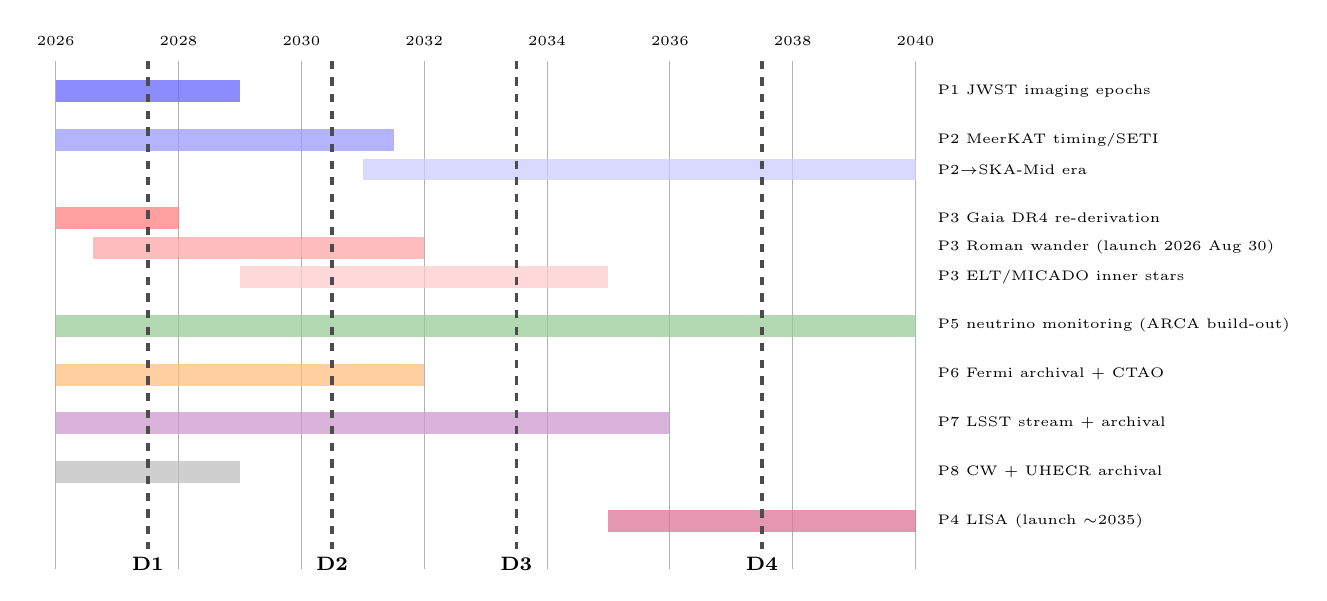
\begin{tikzpicture}[xscale=0.78, yscale=0.62]
% years 2026..2040 mapped to x=0..14
\foreach \x/\yr in {0/2026, 2/2028, 4/2030, 6/2032, 8/2034, 10/2036, 12/2038, 14/2040}
  {\draw[black!30] (\x,0.4) -- (\x,-10.0); \node[font=\tiny] at (\x,0.8) {\yr};}
% bars: \fill[color] (start,row) rectangle (end,row-0.45);
\newcommand{\tlbar}[5]{\fill[#4, opacity=0.75] (#1,#3) rectangle (#2,#3-0.45); \node[font=\tiny, anchor=west] at (14.2,#3-0.22) {#5};}
\tlbar{0}{3}{0}{blue!60}{P1 JWST imaging epochs}
\tlbar{0}{5.5}{-1}{blue!40}{P2 MeerKAT timing/SETI}
\tlbar{5}{14}{-1.6}{blue!20}{P2$\to$SKA-Mid era}
\tlbar{0}{2}{-2.6}{red!50}{P3 Gaia DR4 re-derivation}
\tlbar{0.6}{6}{-3.2}{red!35}{P3 Roman wander (launch 2026 Aug 30)}
\tlbar{3}{9}{-3.8}{red!20}{P3 ELT/MICADO inner stars}
\tlbar{0}{14}{-4.8}{green!50!black!40}{P5 neutrino monitoring (ARCA build-out)}
\tlbar{0}{6}{-5.8}{orange!50}{P6 Fermi archival + CTAO}
\tlbar{0}{10}{-6.8}{violet!40}{P7 LSST stream + archival}
\tlbar{0}{3}{-7.8}{black!25}{P8 CW + UHECR archival}
\tlbar{9}{14}{-8.8}{purple!55}{P4 LISA (launch $\sim$2035)}
% decision points
\foreach \x/\lab in {1.5/D1, 4.5/D2, 7.5/D3, 11.5/D4}
  {\draw[very thick, black!70, dashed] (\x,0.4) -- (\x,-9.6); \node[font=\scriptsize\bfseries, fill=white, inner sep=1pt] at (\x,-9.9) {\lab};}
\end{tikzpicture}
\caption{Campaign timeline against the facility schedule, 2026--2040. Decision points: D1 (2027): Gaia-DR4 re-derivation of the fast-star bound. D2 (2030): five-year pulsar acceleration profile; Roman wander first results. D3 (2033): pre-LISA synthesis --- $H_0$ versus $H_1$ called at available significance. D4 (2037): LISA verdict, if a source is caught.}
\label{fig:timeline}
\end{figure}

% =====================================================================
\section{The decision structure through 2040}
\label{sec:decision}

Figure~\ref{fig:gantt} lays the facility schedule, the program phases, and the D1--D4 decision points on a single time axis; Figure~\ref{fig:tree} then assembles the campaign into a single decision tree, extending the gravitational-wave branch of Paper A's falsification framework backward into the electromagnetic-and-timing era. Rough branch weights are stated where the inputs exist to estimate them; they are planning priors, not forecasts, and we expect D1/D2 to revise them substantially. The tree's light-branch mass cutoff and spin boundary are taken verbatim from Paper A's falsification matrix (Table~3 of \citealt{Swanson2026MTH}, tests T4 and T5); Paper A is the fence owner and no fence is restated independently here.

\begin{figure}[tbp]
\centering

\includegraphics[width=\textwidth]{figs/fC_timeline.pdf}
\caption{Campaign timeline as a Gantt chart, 2026--2040. Top block: the facility schedule (grey), with Gaia DR4 as a diamond marker at 2026 December 2, the two P1 JWST epochs as ticks on the JWST bar, the KM3NeT/ARCA bar ending at the 230-detection-unit build-out, and the LISA bar starting at the $\sim$2035 launch. Middle block: the observing programs P1--P8 (Table~\ref{tab:programs}), coloured as in Figure~\ref{fig:timeline}. Vertical dashed lines: the decision points D1 (2027, Gaia-DR4 frame re-derivation), D2 (2030, five-year timing profile and Roman wander), D3 (2033, pre-LISA synthesis), and D4 (2035+, LISA; Section~\ref{sec:decision}). Bottom strip: the number of simultaneously active facility and program tracks per year. Coverage peaks in 2029, when SKA-Mid and ELT/MICADO come online while the MeerKAT, JWST, and KM3NeT programs are still running; the decisive measurements cluster at D1--D3 and at the LISA window.}
\label{fig:gantt}
\end{figure}

\begin{figure}[tbp]
\centering
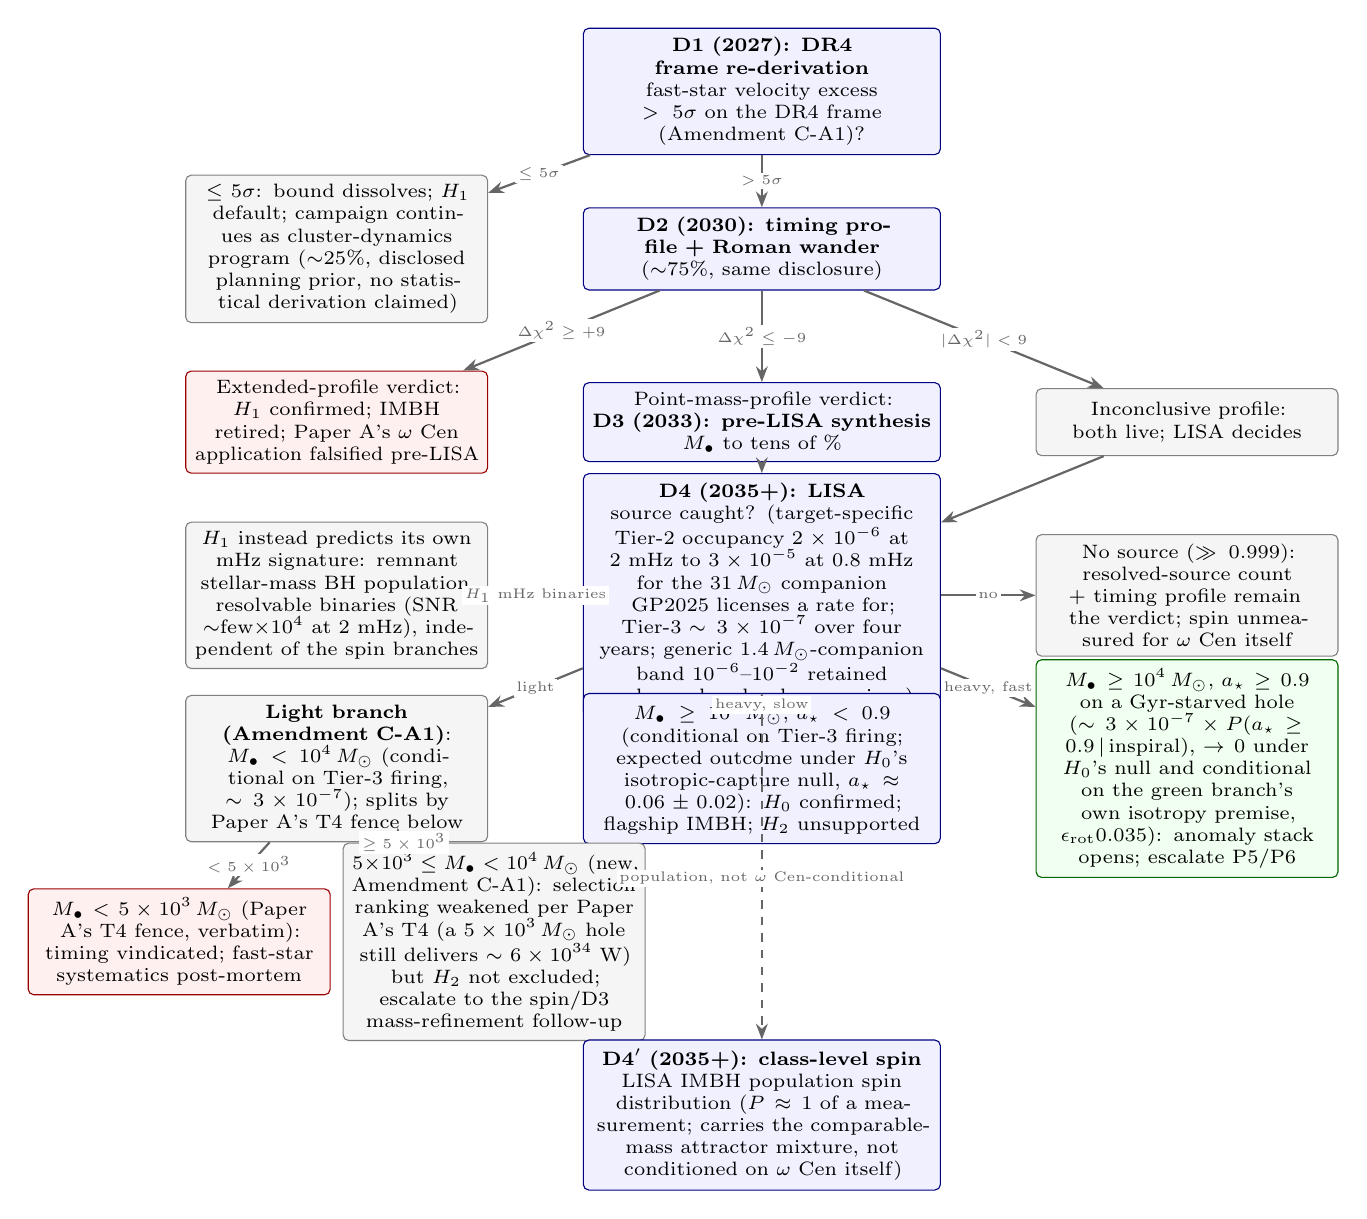
\begin{tikzpicture}[
  q/.style={rectangle, rounded corners=2pt, draw=blue!50!black, fill=blue!6, text width=4.3cm, align=center, font=\scriptsize, minimum height=0.85cm},
  o/.style={rectangle, rounded corners=2pt, draw=black!50, fill=black!4, text width=3.6cm, align=center, font=\scriptsize, minimum height=0.85cm},
  kill/.style={rectangle, rounded corners=2pt, draw=red!60!black, fill=red!6, text width=3.6cm, align=center, font=\scriptsize, minimum height=0.85cm},
  live/.style={rectangle, rounded corners=2pt, draw=green!40!black, fill=green!6, text width=3.6cm, align=center, font=\scriptsize, minimum height=0.85cm},
  arr/.style={-{Stealth[length=2mm]}, thick, black!60},
  lab/.style={font=\tiny, fill=white, inner sep=1pt}
]
\node[q] (d1) at (0,0) {\textbf{D1 (2027): DR4 frame re-derivation}\\ fast-star velocity excess $>5\sigma$ on the DR4 frame (Amendment C-A1)?};
\node[o] (d1no) at (-5.4,-2.0) {$\leq5\sigma$: bound dissolves; $H_1$ default; campaign continues as cluster-dynamics program ($\sim$25\%, disclosed planning prior, no statistical derivation claimed)};
\node[q] (d2) at (0,-2.0) {\textbf{D2 (2030): timing profile + Roman wander} ($\sim$75\%, same disclosure)};
\node[kill] (h1) at (-5.4,-4.2) {Extended-profile verdict: $H_1$ confirmed; IMBH retired; Paper A's $\omega$ Cen application falsified pre-LISA};
\node[q] (d3) at (0,-4.2) {Point-mass-profile verdict:\\ \textbf{D3 (2033): pre-LISA synthesis}\\ $M_{\bullet}$ to tens of \%};
\node[o] (incon) at (5.4,-4.2) {Inconclusive profile: both live; LISA decides};
\node[q] (d4) at (0,-6.4) {\textbf{D4 (2035+): LISA}\\ source caught? (target-specific Tier-2 occupancy $2\times10^{-6}$ at 2~mHz to $3\times10^{-5}$ at 0.8~mHz for the $31\,\msun$ companion GP2025 licenses a rate for; Tier-3 $\sim3\times10^{-7}$ over four years; generic $1.4\,\msun$-companion band $10^{-6}$--$10^{-2}$ retained only as class-level comparison)};
\node[o] (tier1) at (5.4,-6.4) {No source ($\gg 0.999$): resolved-source count + timing profile remain the verdict; spin unmeasured for \ocen{} itself};
\node[o] (hsub) at (-5.4,-6.4) {$H_1$ instead predicts its own mHz signature: remnant stellar-mass BH population, resolvable binaries (SNR $\sim$few$\times10^{4}$ at 2~mHz), independent of the spin branches};
\node[o] (lightgate) at (-5.4,-8.6) {\textbf{Light branch (Amendment C-A1)}: $M_{\bullet} < 10^{4}\,\msun$ (conditional on Tier-3 firing, $\sim3\times10^{-7}$); splits by Paper A's T4 fence below};
\node[q] (midspin) at (0,-8.6) {$M_{\bullet} \geq 10^{4}\,\msun$, $\astar < 0.9$ (conditional on Tier-3 firing; expected outcome under $H_0$'s isotropic-capture null, $\astar \approx 0.06\pm0.02$): $H_0$ confirmed; flagship IMBH; $H_2$ unsupported};
\node[live] (highspin) at (5.4,-8.6) {$M_{\bullet} \geq 10^{4}\,\msun$, $\astar \geq 0.9$ on a Gyr-starved hole ($\sim3\times10^{-7} \times P(\astar\geq0.9\,|\,{\rm inspiral})$, $\to0$ under $H_0$'s null and conditional on the green branch's own isotropy premise, $\epsilon_{\rm rot}\lesssim0.035$): anomaly stack opens; escalate P5/P6};
\node[kill] (small) at (-7.4,-10.8) {$M_{\bullet} < 5\times10^{3}\,\msun$ (Paper A's T4 fence, verbatim): timing vindicated; fast-star systematics post-mortem};
\node[o] (subfloor) at (-3.4,-10.8) {$5\times10^{3} \leq M_{\bullet} < 10^{4}\,\msun$ (new, Amendment C-A1): selection ranking weakened per Paper A's T4 (a $5\times10^{3}\,\msun$ hole still delivers $\sim6\times10^{34}$~W) but $H_2$ not excluded; escalate to the spin/D3 mass-refinement follow-up};
\node[q] (d4p) at (0,-13.0) {\textbf{D4$'$ (2035+): class-level spin}\\ LISA IMBH population spin distribution ($P\approx1$ of a measurement; carries the comparable-mass attractor mixture, not conditioned on \ocen{} itself)};
\draw[arr] (d1) -- (d1no) node[lab, midway] {$\leq5\sigma$};
\draw[arr] (d1) -- (d2) node[lab, midway] {$>5\sigma$};
\draw[arr] (d2) -- (h1) node[lab, midway] {$\Delta\chi^{2}\geq+9$};
\draw[arr] (d2) -- (d3) node[lab, midway] {$\Delta\chi^{2}\leq-9$};
\draw[arr] (d2) -- (incon) node[lab, midway] {$|\Delta\chi^{2}|<9$};
\draw[arr] (d3) -- (d4);
\draw[arr] (incon) -- (d4);
\draw[arr] (d4) -- (tier1) node[lab, midway] {no};
\draw[arr] (d4) -- (hsub) node[lab, midway] {$H_1$ mHz binaries};
\draw[arr] (d4) -- (lightgate) node[lab, midway] {light};
\draw[arr] (d4) -- (midspin) node[lab, midway] {heavy, slow};
\draw[arr] (d4) -- (highspin) node[lab, midway] {heavy, fast};
\draw[arr] (lightgate) -- (small) node[lab, midway] {$<5\times10^{3}$};
\draw[arr] (lightgate) -- (subfloor) node[lab, midway] {$\geq5\times10^{3}$};
\draw[arr, dashed] (d4) -- (d4p) node[lab, midway] {population, not \ocen{}-conditional};
\end{tikzpicture}
\caption{Decision structure through 2040. Red boxes retire hypotheses; the single green branch is the only path on which the technosignature interpretation gains material support, and even there the claim is ``anomaly requiring explanation,'' conditional on the isotropic-capture premise stated on the branch. Percentages and weights are disclosed planning priors rather than computed probabilities, stated at the target-specific rate where GP2025 licenses one; D1's split is binary because any excess at or below the $5\sigma$ contradiction threshold reverts to the same systematics-bias reading, not because a graded middle state was considered and discarded. The colours alone can mislead in two places. First, the fences sit where the experiments are, and not everywhere the mass may be: the $8{,}200\,\msun$ velocity-only lower bound falls inside D4's ``weakened, not falsified'' interval, so a red box on that branch is not an achievable falsification of $H_2$, consistent with the statement in Section~\ref{sec:conclusion} that no null result in this campaign carries evidential weight against $H_2$. Second, the wander and neutrino rows feeding D2 and D3 are systematics-gated rather than decision-grade until their gates are met (the $N$-body scatter floor of Section~\ref{sec:wander} and the window-dependent multiplicity of Section~\ref{sec:neutrino}); where a gate fails, the branch carries no weight and D2 routes on the timing statistic alone. What revises D1's 25/75 weights is stated in advance: a DR4 frame shift that moves the fast-star velocities below the escape speed pushes weight toward the systematics reading, and one that leaves the excess intact at $>5\sigma$ pushes it the other way, so the prior is revised by the size and sign of the frame correction rather than by a judgement call after the fact. D2's routing follows Amendments C-A1 and C-A2 below, sourced to the executed mock forecast (\texttt{paper/figs/fC\_calc7b\_d2forecast\_v2.py}). The routing statistic is the fixed-parameter one, twice the log-likelihood ratio between the two named potentials with no free parameters, signed positive toward the extended component: $\Delta\chi^{2}_{\rm fixed}\geq+9$ (equivalently $\ln K \geq +4.5$, exact for this statistic) routes to the extended branch, $\leq-9$ to the point-mass branch, and $|\Delta\chi^{2}_{\rm fixed}|<9$ to the inconclusive branch. The free-parameter statistic routes nothing, and the point-mass branch is a verdict against the named $2.5\times10^{5}\,\msun$ extended model rather than against extended models in general (Amendment C-A2). D4's light branch now splits at Paper A's T4 fence ($5\times10^{3}\,\msun$), closing the previously uncovered $[5\times10^{3},10^{4})\,\msun$ interval (Amendment C-A1); the new sub-floor node does not retire $H_2$, since Paper A's own T4 language already treats that mass range as weakened, not falsified. D4$'$ is the class-level spin test Paper E identifies as the campaign's most informative measurement; it is not \ocen-conditional and is shown dashed for that reason. Every terminal node is a publishable scientific result about a first-rank astrophysical object.}
\label{fig:tree}
\end{figure}

\subsection{Amendment C-A1 (2026-08-26, pre-data)}
\label{sec:amendmentca1}

An external audit round identified three defects in the decision tree as printed through Draft v2.3: the D4 mass partition left $[5\times10^{3},10^{4})\,\msun$ firing no branch at all, an interval that contains the fast-star kinematic lower bound of $8{,}200\,\msun$; the D2 routing into the extended, point-mass, and inconclusive branches carried only qualitative labels while the upstream mock-forecast gate was already numeric; and D1's binary split disclosed no basis for its 25/75 weights. All three are pre-registered-rule defects, so none is repaired silently, following the disclosure convention of the mass-tension companion's Amendments A1--A5. No observation has yet been scored against the tree: every program in this paper remains pre-D1, and this amendment changes only the tree's own text, not any result.

The repair follows a ratified panel review (\texttt{board/notes/R7-PANEL-DECIDE.md}, brief B-1, option (a)) of three ledger findings (\texttt{C-M5}, \texttt{C-M6}, \texttt{C-t13}). First, the D4 gap is closed by splitting the light branch at Paper A's own T4 fence ($5\times10^{3}\,\msun$, adopted verbatim, not restated independently): masses below it retire $H_2$ as before, and the newly covered $[5\times10^{3},10^{4})\,\msun$ interval is scored as a weakened, not falsified, selection ranking, exactly as Paper A's own T4 language already treats that mass range (a $5\times10^{3}\,\msun$ hole still delivers $\sim6\times10^{34}$~W). Second, the D2 routing adopts the numeric thresholds $\Delta\chi^{2}_{\rm fixed}\geq+9$ (extended), $\leq-9$ (point mass), and $|\Delta\chi^{2}_{\rm fixed}|<9$ (inconclusive), taken from this paper's own pre-registered mock-forecast criterion (Section~\ref{sec:radio}, \texttt{0xAlpha/results/R7-CALC-C2D.md}). Amendment C-A2 below revises what the subscript means and bounds where the rule applies. Third, D1's 25/75 split is left in place but is now stated explicitly as a disclosed planning prior with no claimed statistical derivation, matching this figure's own long-standing caption convention; the binary structure is retained because any excess that fails to survive the DR4 re-derivation at $>5\sigma$ collapses to the same systematics-bias reading regardless of degree, not because a graded middle outcome was considered and discarded.

\subsection{Amendment C-A2 (2026-09-03, pre-data)}
\label{sec:amendmentca2}

Amendment C-A1 named a numeric D2 routing threshold without naming which of the forecast's statistics it applies to, and justified the threshold with an equivalence that holds for only one of them. Re-running the forecast on a corrected joint likelihood (Section~\ref{sec:radio}) shows the ambiguity is not cosmetic: the two statistics route the same data to opposite branches. This amendment fixes the routing statistic, bounds the rule's scope, and records the three defects found in the machinery. As with C-A1, no observation has been scored against the tree; every program remains pre-D1.

\textbf{The routing statistic is the fixed-parameter one.} D2 routes on $\Delta\chi^{2}_{\rm fixed}$, twice the log-likelihood ratio between the two \emph{named} potentials with no free parameters, signed positive toward the extended component. The equivalent evidence band is $\ln K \geq +4.5$ (extended) or $\leq -4.5$ (point mass), and for this statistic alone $\Delta\chi^{2} = 2\ln K$ exactly. The free-parameter statistic, which profiles each family over its own grid, is reported as a diagnostic and routes nothing. Had C-A1's threshold been read on the free-parameter statistic, an injected $2\times10^{4}\,\msun$ point mass would have routed to the extended branch in 82--89 per cent of realizations at every noise floor tested, which is the outcome this amendment exists to prevent.

\textbf{Scope.} The rule adjudicates the two named potentials and nothing else. On the mass-matched third truth of Section~\ref{sec:radio} it misroutes a genuinely extended component to the point-mass branch in 91--100 per cent of realizations once the noise floor reaches $31.6$ (km\,s$^{-1}$)$^{2}$\,pc$^{-1}$, so a D2 verdict of ``point mass'' is a verdict against the named $2.5\times10^{5}\,\msun$ extended model and not against extended models in general. Where the mass-matched cell fails, D2 weight shifts to the astrometric channels of Section~\ref{sec:astrometry} on the same rule C-A1 already states for a short forecast.

\textbf{Machinery defects, disclosed rather than repaired silently.} The v2 script corrects three faults in the executed forecast, and the v1 script is retained so the chain stays auditable. The family fits summed each pulsar's own marginal likelihood over the mass grid, which let every pulsar choose an independent central mass instead of testing one common potential; both the profile maximum and the evidence are now formed on the joint likelihood across pulsars. A unit constant converting (km\,s$^{-1}$)$^{2}$\,pc$^{-1}$ to m\,s$^{-2}$ was wrong by a factor $10^{22}$ and disagreed with its own comment; the correct value is $3.2408\times10^{-11}$. Validation gate G$_{\rm A}$ was reported as failing and the failure was not surfaced, and the gate was itself mis-constructed: it tested a $2\times10^{4}\,\msun$ mass at $|r| = 0.42$~pc including the visible component, against a printed number for a $4\times10^{4}\,\msun$ point mass at $0.3$~pc. With both the constant and the construction repaired the gate reproduces the printed $6\times10^{-8}$~m\,s$^{-2}$ to 3 per cent, and G$_{\rm B}$, previously one-sided and unfailable, now records that the printed $1$--$4\times10^{-9}$~m\,s$^{-2}$ brackets the median of the extended envelope while the envelope itself spans 3.9 decades. The cell results are unaffected by the unit error, since the noise ladder is dimensionless in the same units; the gates were not. A provenance gate confirms the fixed-parameter statistic is unchanged from v1 to $1.3\times10^{-14}$, so every difference between the two runs is attributable to the likelihood repair.

% =====================================================================
\section{Significance conventions across the companion papers}
\label{app:conventions}

The campaign and its companion papers score evidence in four conventions, and a number quoted in one vocabulary must not be silently read in another. This appendix states the four side by side.

\paragraph{Post-trials $p$-values (this paper).} The frequentist false-alarm probability of a trigger after the look-elsewhere correction over the search's windows, frequencies, and positions. The action boundary is $p < 5\times10^{-7}$ per trigger class (Table~\ref{tab:thresholds}), the discovery convention, with cross-channel combinations handled as in Section~\ref{sec:coordination}. It applies to the trigger layer of all eight programs in this paper.

\paragraph{$\ln K$ Bayes factors (Paper E).} The logarithm of the ratio of evidences between two hypotheses, taken by Paper E as $H_{\rm eng}$ against the best astrophysical null. The action bands follow \citet{Kass1995} as pre-registered in Paper E: below $0$ null-favoured, $0$ to $1$ uninformative, $1$ to $3$ anomaly, $3$ to $5$ strong anomaly, and above $5$, sustained across at least two messengers, candidate. The look-elsewhere treatment is structural: likelihoods are always evaluated on the complete campaign record, never on the promoted subset alone, so the selection effect is priced rather than corrected after the fact, and prior sensitivity is reported as a band rather than a point. It applies to Paper E's adjudication layer, acting on whatever this paper's trigger layer promotes.

\paragraph{95 per cent credible upper limits (Paper F).} The Bayesian one-sided credible bound on a parameter, in Paper F the Bondi efficiency $\epsilon_{\mathrm{B}}$ or the dark mass. There is no action band; the limit is the product rather than a decision. The corresponding treatment is prior sensitivity, reported alongside the bound, since a credible limit conditions on the model instead of testing it. It applies to Paper F's quiescent-accretion limits on \ocen{} and on the comparison clusters.

\paragraph{Posterior mass fractions (Paper H).} The fraction of posterior probability in a region of the dark-component mass and scale-radius plane under one normalized model. There is no discovery threshold; the pre-registered criteria are consistency checks, sign stability of the Bayes factor across every prior cell and posterior-predictive adequacy in each cell. The prior-grid sweeps are themselves the sensitivity treatment, and a verdict is quotable only when it survives the full pre-registered cell set. It applies to Paper H's joint fast-star and pulsar fit.

No single convention is privileged; the choice depends on whether the question is ``should we follow up?'' (frequentist), ``what does the evidence support?'' (Bayes factor), ``what is the bound?'' (credible limit), or ``is the model consistent?'' (posterior check).

% =====================================================================
\section{Conclusion}
\label{sec:conclusion}

Omega Centauri in 2026 presents a configuration that observational astronomy rarely supplies: a contested discovery (the Galaxy's best IMBH candidate) whose two strongest constraints formally contradict each other; an electromagnetic silence deep enough to be a result in itself; an essentially untouched technosignature parameter space; and a fleet of new southern and all-sky instruments (Rubin, Roman, Gaia DR4, KM3NeT, CTAO, SKA-Mid, ELT, and ultimately LISA) arriving on the timescale needed to resolve all of it. The campaign presented here is designed to use that conjunction fully.

Its architecture reflects three commitments. First, \emph{dual use}: every program stands as conventional astrophysics (the mass tension, the quiescent-accretion frontier, the MSP dynamical laboratory, the first deep TeV and neutrino limits on a globular cluster), so that no null result is a loss. Second, \emph{conservative sensitivity accounting}: where the obvious measurement fails (direct fast-star acceleration before $\sim$2040), we demonstrate the failure quantitatively and redesign around it, because a program that oversells its tests invites the credibility collapse that has repeatedly damaged this field. Third, \emph{pre-registration}: hypotheses $H_0$/$H_1$/$H_2$, thresholds, confirmation rules, and decision points are fixed in advance, so that whatever the sky delivers (a remnant swarm, a quiet heavy hole, or a genuine anomaly), the inference chain was written down before anyone knew the answer.

The adjudication asymmetry deserves a blunt statement. Under realistic outcomes, this campaign will resolve $H_0$ versus $H_1$; it will neither support nor retire $H_2$ except through the low-probability LISA spin branch or a serendipitous multi-messenger multiplet. No null result carries evidential weight against $H_2$, because the leakage-free and electromagnetically silent predictions of that hypothesis class are compatible with every null the campaign can produce; what the campaign buys for $H_2$ is the pre-registered infrastructure to adjudicate a positive trigger if one ever arrives, and quantitative limits on the specific loud sub-classes (beacons, warm waste heat above the JWST floor, neutrino bursts at predicted strength).

The cost is US\$8.7M across 2026--2040 including 20\% contingency (Table~\ref{tab:cost}), most of it salaries for archival analysis riding on facilities that are funded regardless. The payoff structure is asymmetric in the campaign's favour: the probable outcomes (a resolved mass tension, a characterized central object, the first technosignature limits on $10^{7}$ old stars) are solid science at modest cost, and the improbable outcome (the green branch of Figure~\ref{fig:tree}) would justify the program many thousands of times over. We commit, symmetrically, to the red branches: if the timing profile confirms an extended remnant component, or LISA delivers a light or slowly spinning hole, the anomaly hypotheses retire here without special pleading, and what remains is what was always underneath: the most interesting stellar system in the southern sky, finally measured properly.

% =====================================================================
\section*{Acknowledgements and disclosure}

The author thanks the maintainers of the NASA Astrophysics Data System and arXiv, on which the citation verification for this work relied. \textbf{AI assistance disclosure:} drafting, citation verification, derivation checking, and figure preparation for this manuscript were performed with substantial assistance from a large language model (Claude, Anthropic), under the author's direction; the author reviewed and takes full responsibility for all claims, derivations, and references. Interactive calculators implementing the quantitative material in this paper, together with the underlying per-instrument proposal studies, are available at \url{https://omegacentauri.me}.

\section*{Data availability}

No new observational data were generated for this work. All quantitative claims derive from the cited literature; analysis conventions for the proposed programs will be released with the respective pipeline papers. The pre-registration documents (hypotheses, trigger matrix, thresholds, and analysis plans, as fixed by Tables~\ref{tab:programs} and~\ref{tab:thresholds}) are maintained at \url{https://omegacentauri.me}.

\bibliographystyle{apalike}
\bibliography{references,campaign-extra}

\end{document}
